% !TeX root = main.tex
%-----------------------------------------------%
% Modelo de Lista de Exercícios
%
% Autor: Rodrigo Nascimento (2022-08-12)
%-----------------------------------------------%

\documentclass[
	% -- opções da classe memoir --
	12pt,				% tamanho da fonte
	openright,			% capítulos começam em pág ímpar (insere página vazia caso preciso)
	oneside,			% twoside para impressão em verso e anverso. Oposto a oneside
	a4paper,			% tamanho do papel.
	% -- opções da classe abntex2 --
	%chapter=TITLE,		% títulos de capítulos convertidos em letras maiúsculas
	%section=TITLE,		% títulos de seções convertidos em letras maiúsculas
	%subsection=TITLE,	% títulos de subseções convertidos em letras maiúsculas
	%subsubsection=TITLE,% títulos de subsubseções convertidos em letras maiúsculas
	% -- opções do pacote babel --
	english,			% idioma adicional para hifenização
%	french,				% idioma adicional para hifenização
%	spanish,			% idioma adicional para hifenização
	brazil				% o último idioma é o principal do documento	
]{abntex2}
\selectlanguage{brazil}
%-----------------------------------------------%
% Informações do DOCUMENTO
%-----------------------------------------------%
\instituicao{Universidade do Estado de Santa Catarina -- UDESC}
\titulo{Notas de Mecânica Estatística}
\autor{Rodrigo Nascimento}
\local{Joinville - SC}
\data{\mydate}
\tipotrabalho{Nota de Aula:}
\orientador{Dr. Bruno Duarte da Silva Moreira}
\coorientador{Prof. Me. Supervisor}
%-----------------------------------------------%
% Para alterar o parâmetros dos comandos orientador
% e coorientador.
%-----------------------------------------------%
% \renewcommand{\orientadorname}{Orientadora:}
\renewcommand{\coorientadorname}{Supervisor:}
%-----------------------------------------------%

\newcommand{\centro}{Centro de Ciências Tecnológicas -- CCT }
\newcommand{\departamento}{Departamento de Física -- DFIS}
\newcommand{\curso}{Licenciatura em Física }
\newcommand{\disciplina}{Mecânica Estatística -- OMEE001}
\newcommand{\firstkey}{Introdução aos métodos estatísticos}
\newcommand{\secondkey}{Descrição estatística de sistemas físicos}
\newcommand{\thirdkey}{Termodinâmica}
\newcommand{\fourthkey}{Ensemble microcanônico}


%-----------------------------------------------%

% Todas as indicações de pacotes e configurações estão no arquivo de estilo
% chamado texmodel-udesc.sty.
\usepackage{texmodel-udesc}
% \usepackage{draculatheme}
%--------------------%
% Início do documento
%--------------------%
\begin{document}
% ---------------------------
% Insere o CABEÇALHO (HEADER)
% ---------------------------
\thispagestyle{empty}
\begin{center}
	\begin{minipage}[!]{\linewidth}
        \begin{minipage}[!]{.19\linewidth}
            
\includegraphics[width=\linewidth]{img/logo.png}           
        \end{minipage}
        \begin{minipage}[!]{.8\linewidth}
            \center
            \ABNTEXchapterfont\normalsize\MakeUppercase{\imprimirinstituicao}
            \par
            \vspace*{3pt}                     
            \ABNTEXchapterfont\normalsize\MakeUppercase{\centro}
            \par
            \vspace*{3pt}
            \ABNTEXchapterfont\normalsize\MakeUppercase{\departamento}
            \par
            \vspace*{3pt}           
            \ABNTEXchapterfont\normalsize\MakeUppercase{\disciplina}
        \end{minipage}        
    \end{minipage}
    \par\vspace{0.5cm}
    \rule{\textwidth}{.5pt}   
\end{center}
% -----------------------------
% Insere CAMPO DE IDENTIFICAÇÃO
% -----------------------------   
\noindent \textbf{Aluno(a):} \imprimirautor
\par\noindent \textbf{Professor(a):} \imprimirorientador\hfill{}\textbf{Capítulo(s) Ref.:} VII/VIII  
\par\noindent \textbf{\imprimirtipotrabalho} 003  \hfill{}\textbf{Data:} \imprimirdata\hfill{}\textbf{Fase:} LEF102-08U
\rule{\textwidth}{.5pt}
\bigskip{}
\begin{center}
	\ABNTEXchapterfont\Large\MakeUppercase{\imprimirtitulo}
\end{center}

% Campo para OBERVAÇÕES
\noindent \textbf{Resumo:} Atividade avaliativa baseada no livro do Salinas \cite{SALINAS:2001} para a disciplina de Mecânica Estatística – OMEE001.

\par\noindent \textbf{Palavras chave:} \firstkey; \secondkey; \thirdkey; \fourthkey.
%% ============| INÍCIO |===================
% --------------| Q01 |--------------------
\addcontentsline{toc}{section}{Questão}
\begin{prob}
  Considere a distribuição Gaussiana:
  \begin{align}
    p(x)=\frac{1}{\sqrt{2\pi\sigma^2}}\mathrm{e}^{-\frac{1}{2}\left(\frac{x-\mu}{\sigma}\right)^2}
  \end{align}
  onde $\sigma$ é o desvio padrão e $\mu$ a média. Faça plots de $p(x)$ contra $x$ para:
  \begin{enumerate}[label=\alph *)]
    \item $\mu=0$ e $\sigma=0,1$
    \item $\mu=1$ e $\sigma=0,1$
    \item $\mu=0$ e $\sigma=1$
    \item $\mu=1$ e $\sigma=1$
  \end{enumerate}
  Comente a semelhança e diferença entre os casos.
  \newpage
  \begin{sol}
  \par\noindent As \autoref{fig:gaussianas-1} e \autoref{fig:gaussianas-2}, mostram os gráficos das distribuições gaussianas $p(x)$ cada qual com médias $\mu$ e desvios padrão $\sigma$ indicado.
      \begin{figure}[!htb]
      \centering
      \subfloat[$\mu=0$ \label{fig:figura01}]{
        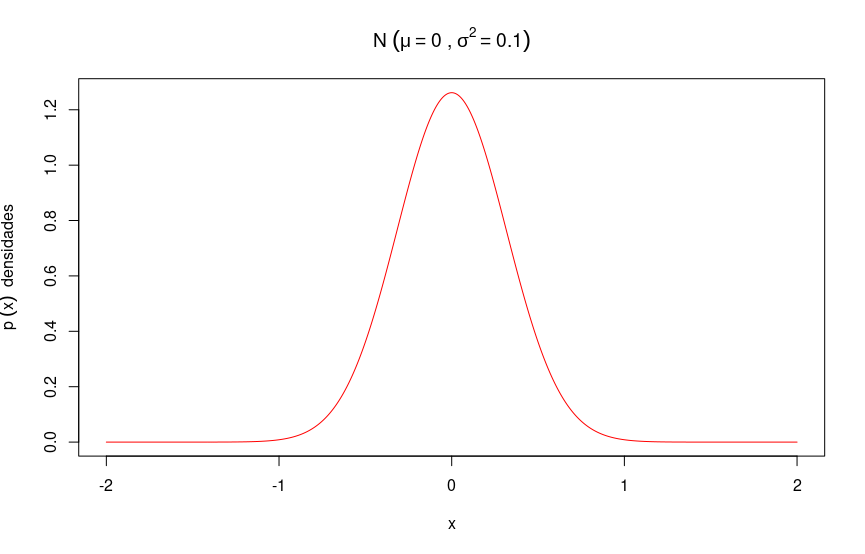
\includegraphics[width=0.48\textwidth]{img/N-m0-s01.png}
      }\hfill
      \subfloat[$\mu=1$ \label{fig:figura02}]{
        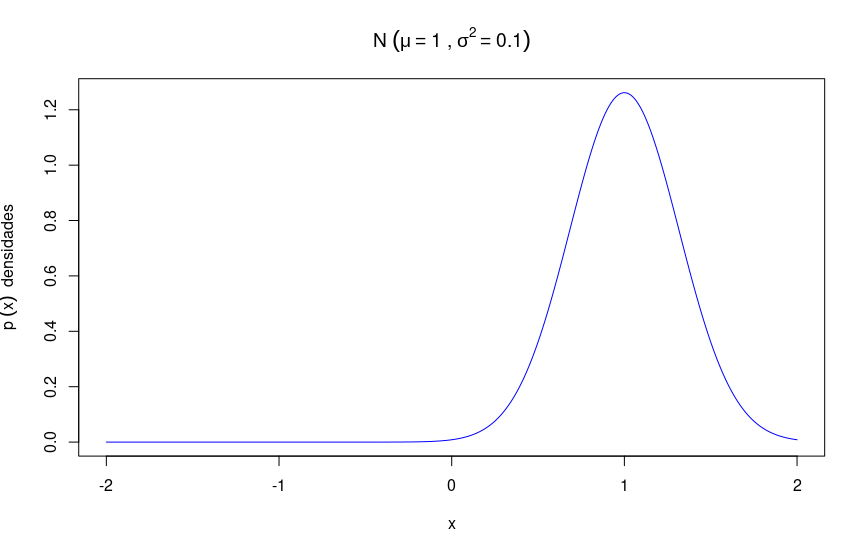
\includegraphics[width=0.48\textwidth]{img/N-mu1-s001.png}
      }        
      \caption{Distribuições gaussianas de mesma variância $\sigma^2=0,01$}
      \label{fig:gaussianas-1}       
    \end{figure}
    \begin{figure}[!htb]
      \centering
      \subfloat[$\mu=0$ \label{fig:figura03}]{
        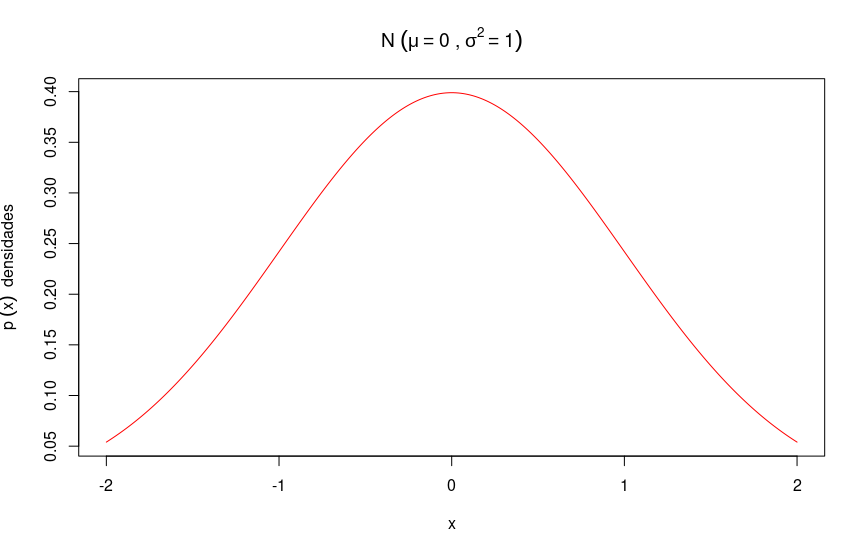
\includegraphics[width=0.48\textwidth]{img/fig-c.png}
      }\hfill
      \subfloat[$\mu=1$ \label{fig:figura04}]{
        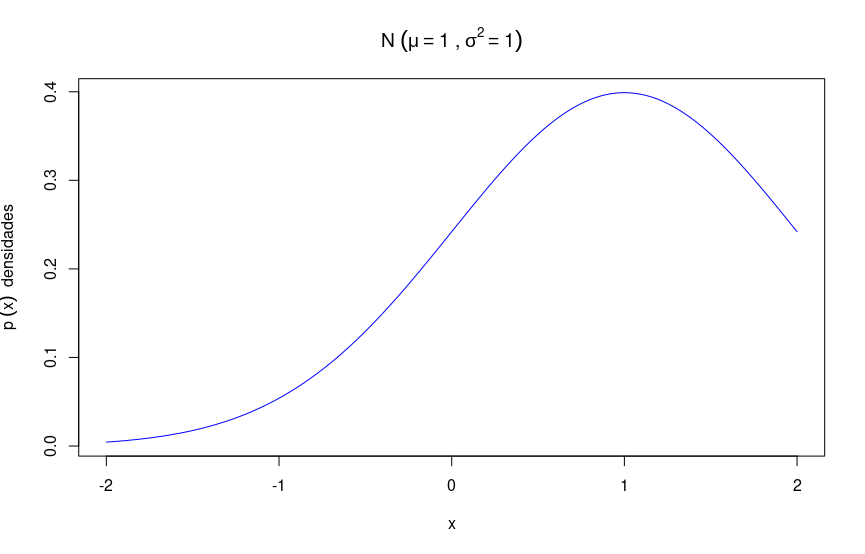
\includegraphics[width=0.48\textwidth]{img/fig-d.png}
      }        
      \caption{Distribuições gaussianas de mesma variância $\sigma^2=1$}
      \label{fig:gaussianas-2}       
    \end{figure}
    \begin{enumerate}[label=\alph *)]
      \item O gráfico da Figura\autoref{fig:figura02} assim como o gráfico da Figura\autoref{fig:figura04}, tem a sua forma deslocada para a direita, com relação aos gráficos da Figura\autoref{fig:figura01} e da Figura\autoref{fig:figura03} respectivamente, indicando que a curva é simétrica com relação a média $\mu$ e consequentemente, uma densidade de probabilidade maior em torno dessa média.
      \item Já os gráficos da \autoref{fig:gaussianas-1} diferem com relação aos gráficos da \autoref{fig:gaussianas-2}, pelo "achatamento" da curva, o que evidencia uma maior dispersão dos valores em torno da média. Quanto maior a variância $\sigma^2$, mais dispersos serão os valores da variável que se enquadra neste tipo de distribuição. 
    \end{enumerate}
  \end{sol}
\end{prob}
% ---------------------------

% -----------------------------
% inserir o sumario
% -----------------------------------------------%
\pdfbookmark[0]{\contentsname}{toc}
\tableofcontents*
\cleardoublepage
% -----------------------------------------------%
% ---------------
% INÍCIO DA LISTA
% ---------------
\textual
%\pagestyle{cabecalholimpo}
\pagestyle{listaex}
% ---------------
% arquivos
%% ============| INÍCIO |===================
% --------------| Q01 |--------------------
\addcontentsline{toc}{section}{Problema 01}
\begin{prob}
Mostre que a expressão para o terceiro momento de uma distribuição binomial $\langle(\Delta N_1)^3 \rangle$ é $Npq(q-p)$
\begin{sol}
Partindo da definição \ref{def:n-momentum}
\begin{definition}[$n$-ésimo momento]
	\label{def:n-momentum}
	O momento de ordem $n$ em relação à média de uma variável aleatória $u$, é dado por:
	\begin{align}
		\label{eq:n-momentum}
		\langle(\Delta u)^n\rangle & =\langle\left(u-\langle u\rangle\right)^n\rangle
	\end{align}
\end{definition}
\noindent Deseja-se demostrar que $\langle\left(\Delta N_1\right)^3\rangle=Npq(q-p)$.
\begin{proof}
	\noindent Partindo da Definição: 0.0.1, tem-se que:
	\begin{align}
		\label{eq:3-momentum}
		\langle\left(\Delta N_1\right)^3\rangle & =\langle\left(N_1-\langle N_1\rangle\right)^3\rangle\nonumber \\
		\langle\left(\Delta N_1\right)^3\rangle & =\langle\left(N_1-\langle N_1\rangle\right)\left(N_1-\langle N_1\rangle\right)^2\rangle\nonumber \\
		\langle\left(\Delta N_1\right)^3\rangle & =\langle\left(N_1-\langle N_1\rangle\right)\left(N_1^2-2N_1\langle N_1\rangle+\langle N_1\rangle^2\right)\rangle\nonumber \\
		\langle\left(\Delta N_1\right)^3\rangle & =\langle N_1^3-3N_1^2\langle N_1\rangle+3N_1\langle N_1\rangle^2-\langle N_1\rangle^3\rangle\nonumber \\
		\langle\left(\Delta N_1\right)^3\rangle & =\langle N_1^3\rangle-3\langle N_1^2\rangle\langle \langle N_1\rangle\rangle+3\langle N_1\rangle\langle\langle N_1\rangle^2\rangle-\langle\langle N_1\rangle^3\rangle\nonumber \\
		\langle\left(\Delta N_1\right)^3\rangle & =\langle N_1^3\rangle-3\langle N_1^2\rangle\langle N_1\rangle+3\langle N_1\rangle\langle N_1\rangle^2-\langle N_1\rangle^3\nonumber \\
		\langle\left(\Delta N_1\right)^3\rangle & =\langle N_1^3\rangle-3\langle N_1^2\rangle\langle N_1\rangle+2\langle N_1\rangle^3
	\end{align}
	Agora, dado que
	\begin{align}
		\label{eq:N1}
		\langle N_1\rangle & =p\parder{}{p}\color{deepblue}{\underbrace{
			\color{black}{\sum_{N_1=0}^N\frac{N!}{N_1!N_2!}p^{N_1}p^{N_2}}
		}_{(p+q)^N}} \nonumber  \\
 		&=p\parder{}{p}\left(p+q\right)^N=pN\CancelTo[\color{deepred}]{p+q=1}{\left(p+q\right)^{N-1}}\nonumber \\
         & =Np
	\end{align}
	e
	\begin{align}
		\label{eq:N2}\langle N_1^2\rangle &=\left(p\parder{}{p}\right)\left\{\left(p\parder{}{p}\right)\left[\sum_{N_1=0}^N\frac{N!}{N_1!N_2!}p^{N_1}q^{N_2}\right]\right\}\nonumber \\
        &=\left(p\parder{}{p}\right)\left[pN\left(p+q\right)^{N-1}\right]\nonumber \\
        &=Np+Np^2\left(N-1\right)\CancelTo[\color{deepred}]{1}{\left(p+q\right)^{N-2}}\nonumber \\
        & =Np+Np^2\left(N-1\right)
	\end{align}
	analogamente tem-se
	\begin{align}
		\label{eq:N3}\langle N_1^3\rangle=\left(p\parder{}{p}\right)&\left(p\parder{}{p}\right)\left\{\left(p\parder{}{p}\right)\left[\sum_{N_1=0}^N\frac{N!}{N_1!N_2!}p^{N_1}q^{N_2}\right]\right\}\nonumber  \\
		=\left(p\parder{}{p}\right)&\left(p\parder{}{p}\right)\left[pN\left(p+q\right)^{N-1}\right]\nonumber \\
		=Np&\left\{\left(\parder{}{p}\right)\left[p\left(p+q\right)^{N-1}+p^2\left(N-1\right)\left(p+q\right)^{N-2}\right]\right\}\nonumber \\
		=Np&\left[\CancelTo[\color{deepred}]{1}{\left(p+q\right)^{N-1}}+p\left(N-1\right)\CancelTo[\color{deepred}]{1}{\left(p+q\right)^{N-2}}+2p\left(N-1\right)\CancelTo[\color{deepred}]{1}{\left(p+q\right)^{N-2}}+\right.\nonumber \\
        &\left.+p^2\left(N-1\right)\left(N-2\right)\CancelTo[\color{deepred}]{1}{\left(p+q\right)^{N-3}}\right]\nonumber \\
        &=Np\left[1+3p\left(N-1\right)+p^2\left(N-1\right)\left(N-2\right)\right]\nonumber \\
        &=Np\left\{1+p\left(N-1\right)\left[3+p\left(N-2\right)\right]\right\}
	\end{align}
	Utilizando os resultados das eqs. (\ref{eq:N1}), (\ref{eq:N2}) e (\ref{eq:N3}) na (\ref{eq:3-momentum}), temos que
	\begin{align}
		\langle\left(\Delta N_1\right)^3\rangle=Np&\left\{1+p\left(N-1\right)\left[3+p\left(N-2\right)\right]\right\}-\nonumber \\
       		   &-3Np\left[Np+Np^2\left(N-1\right)\right]+2N^3p^3\nonumber \\
		=Np&+Np^2\left(N-1\right)\left[3+p\left(N-2\right)\right]-\nonumber \\
       		   &-3N^2p^2-3N^2p^3\left(N-1\right)+2N^3p^3\nonumber \\
		=Np&+Np^2\left[3N-3+p\left(N-1\right)\left(N-2\right)\right]-\nonumber \\
			  -&3N^2p^2-3N^3p^3+3N^2p^3+2N^3p^3\nonumber \\
		=Np&\cancel{+3N^2p^2}-3Np^2+Np^3\left(N^2-3N+2\right)-\nonumber \\
               &\cancel{-3N^2p^2}-N^3p^3+3N^2p^3\nonumber \\
		=Np&-3Np^2\cancel{+N^3p^3}\cancel{-3N^2p^3}+2Np^3-\nonumber \\
               &\cancel{-N^3p^3}\cancel{+3N^2p^3}\nonumber \\
		=Np&-3Np^2+2Np^3\nonumber \\
		=Np&-2Np^2-Np^2+2Np^3\nonumber \\
		=Np&\left(1-2p\right)-Np^2\left(1-2p\right)\nonumber \\
		=Np&\left(1-2p\right)\CancelTo[\color{deepgreen}]{q}{\left(1-p\right)}\nonumber \\
		=Np&q\left(p+q-2p\right)\nonumber \\
		=Np&q\left(q-p\right)
	\end{align}
\end{proof}
\end{sol}
\end{prob}
% --------------| Q02 |--------------------
\newpage
\addcontentsline{toc}{section}{Problema 02}
\begin{prob}
	Uma variável aleatória $x$ está associada à densidade de probabilidade
	\begin{align}
		p(x) & =e^{-x},\qquad  \forall\; x\in \mathbb{R^\ast _+}\nonumber
	\end{align}
	\begin{enumerate}[label=\alph *)]
		\item Mostre que a densidade está normalizada a 1;
		\item Encontre o valor médio $\langle x\rangle$;
		\item Sendo $x_1$ e $x_2$ dois valores escolhidos de forma independente, encontre $\langle x_1+x_2\rangle$ e $\langle x_1x_2\rangle$.
	\end{enumerate}

	\begin{sol}
		\begin{enumerate}[label=\alph *)]
			\item Deseja-se demostrar que
			\begin{align}
				\int_{\mathbb{R^*_+}}p(x)dx & =\int_{\mathbb{R^*_+}}e^{-x}dx=1
			\end{align}
			\noindent Trata-se de uma integral imprópria em $\mathbb{R^*_+}$, portanto, façamos $a\to 0$ e $b\to +\infty$ de modo que tenhamos
			\begin{align}
				\int_{\mathbb{R^*_+}}p(x)dx & =\int_{a}^{b}e^{-x}dx=1
			\end{align}
			\begin{proof}
				\begin{align}
					\label{dem:a}
					\int_{\mathbb{R^*_+}}p(x)dx&=\int_{a}^{b}e^{-x}dx\nonumber \\
				    & =-e^{-x}\Biggr |_a^b\nonumber \\
				    &=e^{-a}-e^{-b}\nonumber \\
				    & =\CancelTo[\color{deepred}]{1}{\lim_{a\to 0}\left(\frac{1}{e^a}\right)}-\CancelTo[\color{deepgreen}]{0}{\lim_{b\to +\infty}\left(\frac{1}{e^b}\right)}\nonumber \\
				    & =1
				\end{align}
			\end{proof}
				\item Por definição definição
				\begin{definition}
					Se $x$ é uma variável aleatória contínua e $f(x)$ a sua função densidade de probabilidade, então:
					\begin{align}
						\label{def:valor-esperado-fdp}
						\langle x\rangle & =\int_{-\infty}^{+\infty}xf(x)dx
					\end{align}
				\end{definition}
				Avaliando primeiramente a integral num intervalo $[a,b]$ temos
				\begin{align}
					\int_{a}^{b}xe^{-x}dx & =-xe^{-x}\Biggr |_a^b+\int_{a}^{b}e^{-x}dx
					\label{eq:x-valor-esperado}
				\end{align}
				se $a\to 0$ e $b\to +\infty$, já vimos na Eq. (\ref{dem:a}) que a integral do lado direito converge e seu valor é 1, então
				\begin{align}
					\int_a^b xe^{-x}dx & =-xe^{-x}\Biggr |_a^{b}+1\nonumber\\
                  	& =1+\lim _{b\to +\infty}\left[(0)(1)-\frac{b}{e^{b}}\right]\nonumber\\
                  	& =1-\CancelTo[\color{deepred}]{0}{\lim _{b\to +\infty}\left(\frac{1}{be^b}\right)}\nonumber\\
                  	& =1
				\end{align}
				portanto
				\begin{align}
					\langle x\rangle & =1
				\end{align}
				\item Note que, dado o enunciado, podemos escrever $\langle x_1+x_2 \rangle=\langle x_1\rangle+\langle x_2\rangle$ e $\langle x_1x_2\rangle=\langle x_1\rangle\langle x_2\rangle$, além disso, da \autoref{eq:x-valor-esperado} sabemos  que $\langle x_1\rangle=1$ e $\langle x_2\rangle=1$, assim
				\begin{align}
					\langle x_2+x_1\rangle=&(1)+(1)=2\\
					\langle x_1\rangle\langle x_2\rangle=& (1)(1)=1
				\end{align}
		\end{enumerate}
	\end{sol}
\end{prob}
% --------------| Q03 |--------------------
\addcontentsline{toc}{section}{Problema 03}
\begin{prob}
	Obtenha o número de microestados acessíveis ao sistema de dois osciladores quânticos
	localizados e independentes, um com frequência fundamental $\omega_0$ e outro com $3\omega_0$, sendo a energia
	total do sistema $10\hbar \omega_0$. Explicite os números quânticos de cada oscilador que levam a esta
	energia total. \textbf{Sugestão: liste todas as possibilidades de números quânticos que levam ao resultado $E,N=10\hbar \omega_0$  (não são muitas!)}
	\begin{sol}
		Sabemos que
		\begin{align}
			E_n&=\left(n+\frac{1}{2}\right)\hbar\omega
		\end{align}
		Para os osciladores $n_1$ e $n_2$ teremos respectivamente
		\begin{align}
			E_{n_1}&=\left(n_1+\frac{1}{2}\right)\hbar\omega_0\\
			E_{n_2}&=\left(n_2+\frac{1}{2}\right)3\hbar\omega_0
		\end{align}
		sabemos também que $E_{1,2}=E_{n_1}+E_{n_2}$, decorre disto que
		\begin{align}
			\label{eq:osciladores-n1n2}
			\begin{split}
				E_{1,2}&=\left(n_1+\frac{1}{2}\right)\hbar\omega_0+\left(n_2+\frac{1}{2}\right)3\hbar\omega_0\\
				E_{1,2}&=n_1\hbar\omega_0+\frac{1}{2}\hbar\omega_0+3n_2\hbar\omega_0+\frac{3}{2}\hbar\omega_0\\
				E_{1,2}&=\left(n_1+3n_2\right)\hbar\omega_0+2\hbar\omega_0
			\end{split}
		\end{align}

		Sendo a energia total do sistema dos dois osciladores $E_{1,2}=10\hbar\omega_0$ então, resolvendo a \eqref{eq:osciladores-n1n2} para $n_2$ e arbitrando o valor de $n_1$ obtemos a tabela
\begin{table}[!ht]
	\centering
	\begin{tabular}{|c|c|c|c|c|c|c|c|c|}
	\hline
	\textbf{$n_1$} & \textbf{$n_1+3n_2=8$} & \textbf{$n_2$} & \textbf{$n_1$} & \textbf{$n_1+3n_2=8$} & \textbf{$n_2$} & \textbf{$n_1$} & \textbf{$n_1+3n_2=8$} & \textbf{$n_2$} \\ \hline
	0              & $0+3n_2=8$            & 8/3            & 3              & $3+3n_2=8$            & 5/3            & 6              & $6+3n_2=8$            & 2/3            \\ \hline
	1              & $1+3n_2=8$            & 7/3            & 4              & $4+3n_2=8$            & 4/3            & 7              & $7+3n_2=8$            & 1/3            \\ \hline
	2              & $2+3n_2=8$            & 2              & 5              & $5+3n_2=8$            & 1              & 8              & $8+3n_2=8$            & 0              \\ \hline
	\end{tabular}
	\caption{Combinações de números quânticos que levam ao valor de energia $E,N=10\hbar\omega_0$}
	\label{tab:numeros-quanticos}
\end{table}

Da tabela \ref{tab:numeros-quanticos}, encontramos 9 possibilidades que resultam na energia total do sistema $E_{1,2}=10\hbar\omega_0$, porém apenas 3 são realmente possíveis ($n_i=0,1,2,...$). Os únicos auto-estados possíveis ($n_1,n_2$) são portanto ($2,2$), (5,1) e (8,0).

Podemos obter o número de micro estados possíveis $\Omega(E,N,N)$ utilizando a relação
\begin{align}
	\label{eq:micro-estados}
	\Omega(E,N)&=\frac{(M+N-1)!}{M!(N-1)!}
\end{align}
Da equação \eqref{eq:osciladores-n1n2} tem-se que $M=n_1+3n_2$, se são 2 osciladores, então $N=2$, e uma vez que
\begin{align}
	E_{n_1,n_2}&=M\hbar\omega_0+\frac{N}{2}\hbar\omega_0
\end{align}
encontramos $M$ em termos da energia tal como segue
\begin{align}
	\begin{split}
		M\hbar\omega_0+2\hbar\omega_0&=E_{1,2}\\
		M\hbar\omega_0&=E_{1,2}-2\hbar\omega_0\\
		M&=\frac{E_{1,2}}{\hbar\omega_0}-2
	\end{split}
\end{align}
substituindo tudo em \eqref{eq:micro-estados}
\begin{align}
	\begin{split}
		\Omega(E,N)&=\frac{\Biggl[\left(\frac{E_{1,2}}{\hbar\omega_0}-2\right)+2-1\Biggr]!}{\left(\frac{E_{1,2}}{\hbar\omega_0}-2\right)!\left(2-1\right)!}\\
		\Omega(E,N)&=\frac{\left(\frac{E_{1,2}}{\hbar\omega_0}-1\right)!}{\left(\frac{E_{1,2}}{\hbar\omega_0}-2\right)!}\\
		\Omega(E,N)&=\frac{\left(\frac{10\hbar\omega_0}{\hbar\omega_0}-1\right)!}{\left(\frac{10\hbar\omega_0}{\hbar\omega_0}-2\right)!}\\
		\Omega(E,N)&=\frac{9!}{8!}\\
		\Omega(E,N)&=9
	\end{split}
\end{align}
Há um total de 9 estados mas somente 3 possíveis como havíamos observado.
	\end{sol}
\end{prob}

% --------------| Q04 |--------------------
\addcontentsline{toc}{section}{Problema 04}
\begin{prob}
	Em um modelo simplificado para um gás de partículas, o volume do sistema é dividido em
	 $V$ células de volume unitário (pode ser tratado como um “número” de volumes). Encontre o 
	 número	de maneiras de distribuir:
	 \begin{enumerate}[label=\alph *)]
	 	\item $N$ partículas distinguíveis $(0\leq N\leq V)$ entre $V$ células de modo que cada célula
	 	possa estar vazia ou ocupada por uma única partícula.
	 	\item Como a resposta é alterada se as partículas forem indistinguíveis?
	 	\item \textbf{Referente ao item b:} considere que $V$ e $N$ sejam muito grandes e defina a variável $v=V/N$.
	 	Utilize a fórmula de Stirling e mostre que
	 	\begin{align}
	 		\frac{1}{N}\ln \Omega&=v\ln v - (v-1)\ln (v-1)
	 	\end{align}
	 \end{enumerate}
\end{prob}

\begin{sol}
	\begin{enumerate}[label=\alph *)]
		\item Dado $N$ o número de partículas distintas do gás, deseja-se arranjá-las em $V$ volumes tal que $V\geq N$.
		
		\par\noindent\emph{modelização:}

		Imaginemos primeiramente 4 partículas $N_j$ distintas, para 7 volumes $V_k$

		\begin{table}[!ht]
			\centering
			\begin{tabular}{|l|l|l|l|l|l|l|}
			\hline
			$V_1$ & $V_2$ & $V_3$ & $V_4$ & $V_5$ & $V_6$ & $V_7$ \\ \hline
			$N_1$ & $N_2$ &       &       & $N_3$ &       & $N_4$ \\ \hline
			\end{tabular}
		\end{table}
		Sendo partículas distinguíveis, a permutação $N_1\longleftrightarrow N_2$ gera um novo arranjo diferente

		\begin{table}[!ht]
			\centering
			\begin{tabular}{|l|l|l|l|l|l|l|}
			\hline
			$V_1$ & $V_2$ & $V_3$ & $V_4$ & $V_5$ & $V_6$ & $V_7$ \\ \hline
			$N_2$ & $N_1$ &       &       & $N_3$ &       & $N_4$ \\ \hline
			\end{tabular}
		\end{table}
		Neste caso, o número de arranjos distintos é dado pela permutação simples de 7 volumes tomados a cada 4 partículas, ou seja $_7P_4$
		\begin{align}
			_7P_4&=\frac{7!}{(7-4)!}=840
		\end{align}
		Logo, para $V$ volumes e $N$ partículas, temos simplesmente
		\begin{align}
			_VP_N&=\frac{V!}{(V-N)!}
		\end{align}
		portanto,
		\begin{align}
			\Omega (V,N)&=\frac{V!}{(V-N)!}
		\end{align}
			\item Caso as partículas sejam indistinguíveis, então as permutações $N\longleftrightarrow N$ não mais geram novos arranjos, como podemos perceber a seguir
			
			\begin{table}[!ht]
				\centering
				\begin{tabular}{|l|l|l|l|l|l|l|}
				\hline
				$V_1$ & $V_2$ & $V_3$ & $V_4$ & $V_5$ & $V_6$ & $V_7$ \\ \hline
				$N$   & $N$   &       &       & $N$   &       & $N$   \\ \hline
				\end{tabular}
			\end{table}
			e o número de arranjos possíveis, para o caso dos 7 volumes e 4 partículas é dado pela combinação $7\choose 4$, isto é
			\begin{align}
				7C_4&={7\choose 4}=\frac{7!}{(7-4)!4!}=35
			\end{align}
			um número bem menor de arranjos! Generalizando para $V$ volumes e $N$ partículas indistinguíveis teremos
			\begin{align}
				\label{eq:N-indist}
				\Omega (V,N)&=\frac{V!}{(V-N)!N!}
			\end{align}
			\item Pela fórmula de \emph{stirling} tem-se que
			\begin{align}
				\ln \N!&=N\ln N -N+O(\ln N)
			\end{align}
			aplicando o logaritmo natural em ambos os lados da \eqref{eq:N-indist}, obtêm-se
			\begin{align}
				\begin{split}
					\label{eq:aprox-stirling0}
					\ln \Omega&=\ln\left[\frac{V!}{(V-N!)N!}\right]\\
					&=\ln V!-\biggl[\ln\left(V-N\right)!+\ln N!\biggr]	
				\end{split}				
			\end{align}
			usando a série assintótica de stirling em \eqref{eq:aprox-stirling0}	
			\begin{equation}
				\label{eq:aprox-stirling1}
				\begin{split}
					\ln \Omega(V,N)=V\ln V&-\cancel{V}-\Bigl[\left(V-N\right)\ln\left(V-N\right)-\left(\cancel{V}-\cancel{N}\right)+\\
					&+N\ln N-\cancel{N}\Bigr]+O\left(\ln V\right)+O\left[\ln (V-N)\right]+\\
					&+O\ln\left(N\right)
				\end{split}
			\end{equation}
			Tomando $N$ e $V$ suficientemente grandes, podemos descartar os termos da ordem de $\ln$ da série de stirling, ficando apenas com os primeiros termos, além disso, usando $v=V/N$ na \eqref{eq:aprox-stirling1} ficamos com
			\begin{proof}
				\begin{align}
					\begin{split}
						\ln\Omega(v,N)=vN\ln vN&-\Bigl[\left(vN-N\right)\ln\left(vN-N\right)+N\ln N\Bigr]\\
						=vN\ln v+&vN\ln N-\Bigl\{N\left(v-1\right)\ln \Bigl[N\left(v-1\right)\Bigr]+N\ln N\Bigr\}\\
						=N\Bigl\{v\ln v&+\cancel{v\ln N}-\Bigl[\cancel{\left(v-1\right)\ln N}+\left(v-1\right)\ln (v-1)\Bigr]+\cancel{\ln N}\Bigr\}\\
						=N\Bigl[v\ln v&-\left(v-1\right)\ln\left(v-1\right)\Bigr]		
					\end{split}
				\end{align}
				e por fim, dividindo-se ambos os lados da igualdade por $N$, chegamos em
				\begin{align}
						\frac{1}{N}\ln\Omega(v,N)=v\ln v-&\left(v-1\right)\ln\left(v-1\right)
				\end{align}
			\end{proof}
	\end{enumerate}
	
\end{sol}
% --------------| Q05 |--------------------
\addcontentsline{toc}{section}{Problema 05}
\begin{prob}
	A partir da equação de van der Waals
	\begin{align}
		p&=\frac{RT}{v-b}-\frac{a}{v^2}
	\end{align}
	e sabendo que
	\begin{align}
		\label{eq:calor-especifico-vcte}
		c_V&=T\left(\parder{s}{T}\right)_v=c
	\end{align}
	Obtenha a relação fundamental na representação de Helmholtz $f(T,v)$. Logo após, mostre que a densidade de energia é dada por
	\begin{align}
		u&=cT-\frac{a}{v}
	\end{align}
	\begin{sol}
		Partindo da relação
		\begin{align}
			\label{eq:5.1}
			F&=U-TS
		\end{align}
		tem-se que
		\begin{align}
			\label{eq:5.2}
			\begin{split}
				dF&=dU-d(TS)\\
				dF&=dU-TdS-SdT
			\end{split}
		\end{align}
		Escrevendo a 1ª Lei da termodinâmica para o problema
		\begin{align}			
			dU&=TdS-pdV
			\label{eq:1-lei-termodinamica}
		\end{align}
		e utilizando na \eqref{eq:5.2}
		\begin{align}
			\begin{split}
				df&=\color{deepgreen}{\underbrace{\color{black}{(TdS-PdV)}}_{dU}}\color{black}{-TdS-SdT}\\
				dF&=-SdT-pdV
				\label{eq:5.3}
			\end{split}
		\end{align}
		fazendo $s=S/N$ e $v=V/N$
		\begin{align}
			df(T,v)=-sdT-pdv
			\label{eq:5.4}
		\end{align}
		De modo geral, uma diferencial exata pode sempre ser escrita da seguinte forma
		\begin{align}
			\label{eq:5.41}
			df(T,v)&=\left(\parder{f}{T}\right)_vdT+\left(\parder{f}{v}\right)_Tdv
		\end{align}
		resulta da \eqref{eq:5.4} e da \eqref{eq:5.41} que
		\begin{subequations}
			\begin{align}					
					\left(\parder{f}{T}\right)_v&=-s\label{eq:5.5a}\\
					\left(\parder{f}{v}\right)_T&=-p\label{eq:5.5b}
			\end{align}
		\end{subequations}
		reescrevendo a \eqref{eq:5.4} em termos das variáveis do problema
		\begin{align}
			\label{eq:5.6}
			df(T,v)=-sdT+\left(\frac{a}{v^2}-\frac{RT}{v-b}\right)dv
		\end{align}
		Precisamos construir a função $s=s(T,v)$. Assumindo que estas funções possuam também segundas derivadas definidas, a condição de diferenciabilidade exige que
		\begin{align}
			\left[\parder{}{v}\left(\parder{f}{T}\right)_v\right]_T&=\left[\parder{}{T}\left(\parder{f}{v}\right)_T\right]_v
		\end{align}
		essa condição aplicada as \eqref{eq:5.5a} e \eqref{eq:5.5b}, reduz a
		\begin{subequations}
			\begin{align}
				\left[\parder{}{v}\left(\parder{f}{T}\right)_v\right]_T&=-\left(\parder{s}{v}\right)_T \label{eq:cond-diferenciabilidde-s}\\			
				\left[\parder{}{T}\left(\parder{f}{v}\right)_T\right]_v&=-\left(\parder{p}{T}\right)_v \label{eq:cond-diferenciabilidde-p}
			\end{align}
		\end{subequations}
		observe que $s=s(T,v)$, é
		\begin{align}
			\label{eq:derivada-funcao-s}
			ds(T,v)&=\left(\parder{s}{v}\right)_Tdv+\left(\parder{s}{T}\right)_vdT
		\end{align}
		Achar a $(\partial_vs)_T$, é simples, basta utilizar a condição de diferenciabilidade expressa pelas relações \eqref{eq:cond-diferenciabilidde-s} e \eqref{eq:cond-diferenciabilidde-p}, de modo que
		\begin{align}
			\left(\parder{s}{v}\right)_T&=\left(\parder{p}{T}\right)_v
		\end{align} 
		i.e.:
		\begin{align}
			\begin{split}
				\label{eq:s-funcao-v}
				\left(\parder{s}{v}\right)_T&=\left[\parder{}{T}\left(\frac{RT}{v-b}-\frac{a}{v^2}\right)\right]\\
				\left(\parder{s}{v}\right)_T&=\frac{R}{v-b}
			\end{split}
		\end{align}
		agora, a relação $(\partial_Ts)_v$ é dada pelo problema [vide eq.:\eqref{eq:calor-especifico-vcte}], atualizando a \eqref{eq:derivada-funcao-s} tem se
		\begin{align}
			ds(T,v)&=\left(\frac{R}{v-b}\right)dv+\frac{c_v}{T}dT
		\end{align}
		cujo a solução é conhecida, pelo o que segue
		\begin{align}
			\begin{split}
				s(v,T)&=\int_{v}\left(\frac{R}{v-b}\right)dv+g(T)\\
				s(v,T)&=R\ln(v-b)+g(T)\\
				\left(\parder{s}{T}\right)_T&=\frac{dg(T)}{dT}=\frac{c_v}{T}\implies g(T)=c_v\ln T								
			\end{split}
		\end{align}
		\begin{align}
			\boxed{
					s(v,T)=R\ln (v-b)+c_v\ln T
				}
		\end{align}
		procedendo de forma semelhante com a \eqref{eq:5.6} obtemos
		\begin{align}
			\begin{split}
				f(v,T)&=-\left[R\ln (v-b)+c_v\ln T\right]dT+\left(\frac{a}{v^2}-\frac{RT}{v-b}\right)dv\\
				f(v,T)&=-\int_T\left[R\ln(v-b)+c_v\ln T\right]dT+h(v)\\
				f(v,T)&=-RT\ln(v-b)-c_vT(\ln T-1)+h(v)\\
				\left(\parder{f}{v}\right)_T&=-\frac{RT}{v-b}+\frac{dh(v)}{dv}=\frac{a}{v^2}-\frac{RT}{v-b}\implies h(v)=-\frac{a}{v}
			\end{split}			
		\end{align}
		a relação fundamental da equação de van der Waals na representação de Helmholtz $f(T,v)$, fica
		\begin{align}
			\boxed{
				f(v,T)=-RT\ln(v-b)-c_vT(\ln T-1)-\frac{a}{v}
			}
		\end{align}
		Tendo encontrado $f$ e $s$, obtêm-se a representação em termos da densidade de energia bastando fazer
		\begin{align}
			u&=f+Ts
		\end{align}
		na \eqref{eq:5.1}, logo
		\begin{align}
			\begin{split}
				u&=-RT\ln(v-b)-c_vT(\ln T-1)-\frac{a}{v}+T\left[R\ln (v-b)+c_v\ln T\right]\\
				u&=\cancel{-RT\ln(v-b)}\cancel{-c_vT\ln T}+c_vT-\frac{a}{v}\cancel{+TR\ln (v-b)}\cancel{+Tc_v\ln T}
			\end{split}
		\end{align}
		\begin{align}
			\boxed{
				u=c_v-\frac{a}{v}
			}
		\end{align}
	\end{sol}
\end{prob}
% --------------| Q06 |--------------------
\addcontentsline{toc}{section}{Problema 06}
\begin{prob}
	Considere um fluido puro de uma componente. Utilize as relações de Maxwell na representação
de Helmholtz para mostrar que
\begin{align}
	\label{eq:relacao-prob6.1}
	\left(\parder{s}{v}\right)_T&=\left(\parder{p}{T}\right)_v
\end{align}
Com este resultado, mostre que
\begin{align}
	\label{eq:relacao-prob6.2}
	\left(\parder{c_v}{v}\right)_T&=T\left(\parder{^2p}{T^2}\right)_v
\end{align}
\begin{sol}
	Considere a representação de Helmholtz na forma diferencial
	\begin{align}
		\label{eq:representacao-helmholtz}
		dF&=-SdT-pdV+\mu dN
	\end{align}
	As relações de Maxwell na representação de Helmholtz, decorrem da condição de existência da função $F(T,V,N)$ e de suas derivadas, como já visto no problema anterior, uma vez que podemos escrever
	\begin{align}
		\label{eq:representacao-helholtz-delparc}
		dF(T,V,N)&=\left(\parder{F}{T}\right)_{V,N}dT+\left(\parder{F}{V}\right)_{T,N}dV+\left(\parder{F}{N}\right)_{T,V}dN
	\end{align}
	a condição de existência das derivadas primeiras e segundas, necessita que
	\begin{subequations}
		\begin{align}
			\left[\parder{}{V}\left(\parder{F}{T}\right)_{V,N}\right]_{T,N}=\left[\parder{}{T}\left(\parder{F}{V}\right)_{T,N}\right]_{V,N}\label{eq:d2fdvdt=d2fdtdv}\\
			\left[\parder{}{N}\left(\parder{F}{T}\right)_{V,N}\right]_{T,V}=\left[\parder{}{T}\left(\parder{F}{N}\right)_{T,V}\right]_{V,N}\label{eq:d2fdndt=d2fdtdn}\\
			\left[\parder{}{N}\left(\parder{F}{V}\right)_{T,N}\right]_{T,V}=\left[\parder{}{V}\left(\parder{F}{N}\right)_{T,V}\right]_{T,N}\label{eq:d2fdndv=d2fdvdn}
		\end{align}
	\end{subequations}
	o que combinado com as expressões \eqref{eq:representacao-helmholtz} e \eqref{eq:representacao-helholtz-delparc} resulta diretamente nas relações de Maxwell	
	\begin{subequations}
		\begin{align}
			-\left[\parder{S}{V}\right]_{T,N}&=-\left[\parder{p}{T}\right]_{V,N}\label{eq:maxwell-helmholtz-ps}\\
			-\left[\parder{S}{N}\right]_{T,V}&=\left[\parder{\mu}{T}\right]_{V,N}\label{eq:maxwell-helmholtz-sm}\\
			-\left[\parder{p}{N}\right]_{T,V}&=\left[\parder{\mu}{V}\right]_{T,N}\label{eq:maxwell-helmholtz-pm}
		\end{align}
	\end{subequations}
	Assim, a relação \eqref{eq:relacao-prob6.1} fica justificada pelas relações \eqref{eq:d2fdvdt=d2fdtdv} e \eqref{eq:maxwell-helmholtz-ps}, quando tomadas sobre as densidades $v=V/N$ e $s=S/N$
	\begin{align}
		\left(\parder{s}{v}\right)_{T}&=\left(\parder{p}{T}\right)_{v}
	\end{align}
	tomando a $\partial_T$ em ambos os lados da igualdade acima, tem-se
	\begin{align}
		\left[\parder{}{T}\left(\parder{s}{v}\right)_T\right]_{v}=\left[\parder{}{T}\left(\parder{p}{T}\right)_v\right]_v
	\end{align}
	ou, equivalentemente
	\begin{align}
		\left[\parder{}{v}\left(\parder{s}{T}\right)_v\right]_T=\left(\parder{^2p}{T^2}\right)_v
	\end{align}
	mas $T(\partial_Ts)_v=c_v$, então, multiplicando ambos lados da igualdade acima por $T$ tem-se o que deseja-se demonstrar
	\begin{align}
		\begin{split}
			\left[\parder{}{v}T\left(\parder{s}{T}\right)_v\right]_T&=T\left(\parder{^2p}{T^2}\right)_v\\
			\left(\parder{c_v}{v}\right)&=T\left(\parder{^2p}{T^2}\right)_v\
		\end{split}
	\end{align}
\end{sol}
\end{prob}

% --------------| Q07 |--------------------
\addcontentsline{toc}{section}{Problema 07}
\begin{prob}
	Para o problema do paramagneto de spin $1/2$, partindo da entropia obtida em aula, mostre que:
	\begin{enumerate}[label=\alph *)]
		\item
		\begin{align}
			\frac{1}{T}&=\frac{k_B}{2\mu_0H}\Biggl[\ln\left(1-\frac{u}{\mu_0H}\right)-\ln\left(1+\frac{u}{\mu_0H}\right)\Biggr]			
		\end{align}
		\item
		\begin{align}
			u&=-\mu_0H\tanh\left(\frac{\mu_0H}{k_BT}\right)			
		\end{align}
		\item Utilizando a relação entre densidade de energia e magnetização, obtenha a suscetibilidade
		magnética
		\begin{align}
			\chi(T,H)&=\left(\parder{m}{H}\right)_T=\frac{\mu_0^2}{k_BT}\cosh^{-2}\frac{\mu_0H}{k_BT}
		\end{align}
	\end{enumerate}
	\begin{sol}Em sala de aula, obtemos para a densidade de entropia a seguinte expressão
		\begin{align}
			s(u)&=k_B\ln 2-\frac{k_B}{2}\left(1-\frac{u}{\mu_0H}\right)\ln\left(1-\frac{u}{\mu_0H}\right)-\frac{k_B}{2}\left(1+\frac{u}{\mu_0H}\right)\ln\left(1+\frac{u}{\mu_0H}\right)
		\end{align}
		\begin{enumerate}[label=\alph *)]
			\item Basta avaliarmos $\partial_u s(u)$, sendo assim
			\begin{proof}[Demostração 7(a)]
				\begin{align}
					\label{eq:7A}
					\begin{split}
						\frac{1}{T} = \parder{s(u)}{u}=-\frac{k_B}{2} \Bigg[ \Bigg. & 
						-\left(\frac{1}{\mu_0H}\right)\ln\left(1-\frac{u}{\mu_0H}\right) + \\
						& + \CancelTo[\color{deepgreen}]{1}{\left(1-\frac{u}{\mu_0H}\right)\left(1-\frac{u}{\mu_0H}\right)^{-1}}\left(-\frac{1}{\mu_0H}\right) + \\
						& +\CancelTo[\color{deepgreen}]{1}{\left(1+\frac{u}{\mu_0H}\right)\left(1+\frac{u}{\mu_0H}\right)^{-1}} \left(\frac{1}{\mu_0H}\right) + \\
						& + \left(\frac{1}{\mu_0H}\right)\ln\left(1+\frac{u}{\mu_0H}\right)
						\Bigg. \Bigg]\\
						\frac{1}{T}=\frac{k_B}{2\mu_0H}\Bigg[&\ln\left(1-\frac{u}{\mu_0H}\right)-\ln\left(1+\frac{u}{\mu_0H}\right)\cancel{+1-1} \Bigg]\\
						\frac{1}{T}=\frac{k_B}{2\mu_0H}\Bigg[&\ln\left(\frac{\mu_0H-u}{\mu_0H+u}\right)\Bigg]
					\end{split}
				\end{align}
			\end{proof}
			\item Agora basta invertermos a \eqref{eq:7A}, rearranjando os termos
			\begin{align}				
				\begin{split}
						\frac{1}{T}&=\frac{k_B}{2\mu_0H}\left[\ln\left(\frac{\mu_0H-u}{\mu_0H+u}\right)\right]\\
						\frac{2\mu_0H}{k_BT}&=\ln\left(\frac{\mu_0H-u}{\mu_0H+u}\right)
				\end{split}
			\end{align}
			ou
			\begin{align}				
				\beta&=\frac{1}{k_BT} & \alpha&=\mu_0H				
			\end{align}
			\begin{align}
				\label{eq:7B0}
				2\beta\alpha&=\ln\left(\frac{\alpha-u}{\alpha+u}\right)
			\end{align}
			\begin{proof}[Demostração 7(b)]
				Aplicando a inversa do logaritmo natural em \eqref{eq:7B0} 
				\begin{align}
					\label{eq:7B}
					\begin{split}
						e^{2\alpha\beta}&=\frac{\alpha-u}{\alpha+u}\\
						e^{2\alpha\beta}\left(\alpha+u\right)&=\alpha-u\\
						\alpha e^{2\alpha\beta}+ue^{2\alpha\beta}&=\alpha-u\\
						ue^{2\alpha\beta}+u&=\alpha-\alpha e^{2\alpha\beta}\\
						u\left(e^{2\alpha\beta}+1\right)&=\alpha\left(1-e^{2\alpha\beta}\right)\\
						u&=\alpha\left(\frac{1-e^{2\alpha\beta}}{1+e^{2\alpha\beta}}\right)\left(\frac{-e^{-\alpha\beta}}{-e^{-\alpha\beta}}\right)\\
						u&=-\alpha\left[\frac{-e^{-\alpha\beta}\left(1-e^{2\alpha\beta}\right)}{e^{-\alpha\beta}\left(1+e^{2\alpha\beta}\right)}\right]\\
						u&=-\alpha\left(\frac{e^{-\alpha\beta}-e^{\alpha\beta}}{e^{-\alpha\beta}+e^{\alpha\beta}}\right)\\
						u&=-\alpha\tanh(\alpha\beta)\\
						u&=-\mu_0H\tanh\left(\frac{\mu_0H}{k_BT}\right)
					\end{split}
				\end{align}
			\end{proof}
			\item Considerando que
			\begin{align}
				\begin{split}
					m&=-\frac{u}{H}\\
					m&=\mu_0\tanh\left(\frac{\mu_0H}{k_BT}\right)
				\end{split}
			\end{align}
			e utilizado $d/dx\tanh(x)=\cosh^{-2}(x)$. Basta avaliarmos $\partial_Hm$, como segue
			\begin{align}
				\begin{split}					
				\chi(T,H)&=\left(\parder{m}{H}\right)_T\\
				\chi(T,H)&=\parder{}{H}\left[\mu_0\tanh\left(\frac{\mu_0H}{k_BT}\right)\right]\\
				\chi(T,H)&=\mu_0\left[\cosh^{-2}\left(\frac{\mu_0H}{k_BT}\right)\right]\left(\frac{\mu_0}{k_BT}\right)\\
				\chi(T,H)&=\frac{\mu_0^2}{k_BT}\cosh^{-2}\left(\frac{\mu_0H}{k_BT}\right)
				\end{split}
			\end{align}
		\end{enumerate}
	\end{sol}
\end{prob}

% --------------| Q08 |--------------------
\addcontentsline{toc}{section}{Problema 08}
\begin{prob}
	Partindo da expressão para o número de microestados acessíveis do sólido de Einstein
	\begin{align}
		\Omega(E,N)&=\frac{\left(\frac{E}{\hbar\omega}+\frac{N}{2}-1\right)!}{\left(\frac{E}{\hbar\omega}-\frac{N}{2}\right)!\left(N-1\right)!}
	\end{align}
	obtenha a densidade de entropia do sólido de Einstein.
	\begin{sol}
		Dado a densidade de entropia, como
		\begin{align}
			\label{eq:post-entropia}
			s(u)&=\displaystyle \lim_{N \to \infty;\frac{E}{N}=u}\frac{1}{N}k_B\ln\Omega(E,N)
		\end{align}
		Vamos primeiro aplicar o logaritmo ao número de microestados acessíveis $\Omega(E,N)$
		\begin{align}
			\label{eq:dens-entropia-sol-einstein}
			\begin{split}
				\ln\Omega(E,N)&=\ln\Biggl[\frac{\left(\frac{E}{\hbar\omega}+\frac{N}{2}-1\right)!}{\left(\frac{E}{\hbar\omega}-\frac{N}{2}\right)!\left(N-1\right)!}\Biggr]\\
				&=\ln\left(\frac{E}{\hbar\omega}+\frac{N}{2}-1\right)!-\biggl[\ln\left(\frac{E}{\hbar\omega}-\frac{N}{2}\right)!+\ln\left(N-1\right)\biggr]!
			\end{split}
		\end{align}
		Usando a expansão de stirling em \eqref{eq:dens-entropia-sol-einstein}
		\begin{align}
			\begin{split}
				\ln\Omega(E,N)=&\left(\frac{E}{\hbar\omega}+\frac{N}{2}-1\right)\ln\left(\frac{E}{\hbar\omega}+\frac{N}{2}-1\right)-\left(\frac{E}{\hbar\omega}+\frac{N}{2}-1\right)+\\
				&\qquad-\Biggl[\left(\frac{E}{\hbar\omega}-\frac{N}{2}\right)\ln\left(\frac{E}{\hbar\omega}-\frac{N}{2}\right)-\left(\frac{E}{\hbar\omega}-\frac{N}{2}\right)+\\&\qquad\qquad+\left(N-1\right)\ln\left(N-1\right)-\left(N-1\right)\Biggr]\\
				\ln\Omega(E,N)=&\left(\frac{E}{\hbar\omega}+\frac{N}{2}-1\right)\ln\left[N\left(\frac{E}{N\hbar\omega}+\frac{1}{2}-\frac{1}{N}\right)\right]-\left(\frac{E}{\hbar\omega}-\frac{N}{2}\right)\times\\&\quad\times\ln\left[N\left(\frac{E}{N\hbar\omega}-\frac{1}{2}\right)\right]-(N-1)\ln\left[N\left(1-\frac{1}{N}\right)\right]-\cancel{\left(\frac{E}{\hbar\omega}+{\frac{N}{2}}-{1}\right)}+\\
				&\qquad+\cancel{\left(\frac{E}{\hbar\omega}-\frac{N}{2}\right)+(N-1)}\\
				\ln\Omega(E,N)=&\left(\frac{E}{\omega\hbar}+\frac{N}{2}-1\right)\left[\ln N+\ln\left(\frac{E}{N\hbar\omega}+\frac{1}{2}-\frac{1}{N}\right)\right]-\left(\frac{E}{\hbar\omega}-\frac{N}{2}\right)\times\\&\quad\times\left[\ln N+\ln\left(\frac{E}{N\omega\hbar}-\frac{1}{2}\right)\right]-(N-1)\left[\ln N+\ln\left(1-\frac{1}{N}\right)\right]\\
				\ln\Omega(E,N)=&\left(\frac{E}{\omega\hbar}+\frac{N}{2}-1\right)\ln\left(\frac{E}{N\omega\hbar}+\frac{1}{2}-\frac{1}{N}\right)-\left(\frac{E}{\hbar\omega}-\frac{N}{2}\right)\ln\left(\frac{E}{N\omega\hbar}-\frac{1}{2}\right)+\\&\quad-(N-1)\ln\left(1-\frac{1}{N}\right)+\cancel{\left(\frac{E}{\omega\hbar}+\frac{N}{2}-1\right)\ln N}-\cancel{\left(\frac{E}{\hbar\omega}-\frac{N}{2}\right)\ln N}+\\&\qquad-\cancel{(N-1)\ln N}
			\end{split}
			\label{eq:ln-Omega}
		\end{align}
		dividindo \eqref{eq:ln-Omega} por $N$ obtêm-se
		\begin{align}
			\label{eq:omega-div-n}
			\begin{split}
				\frac{1}{N}\ln\Omega(E,N)=&\left(\frac{E}{N\hbar\omega}+\frac{1}{2}-\frac{1}{N}\right)\ln\left(\frac{E}{N\hbar\omega}+\frac{1}{2}-\frac{1}{N}\right)-\left(\frac{E}{N\hbar\omega}-\frac{1}{2}\right)\times\\&\quad\times\ln\left(\frac{E}{N\hbar\omega}-\frac{1}{2}\right)-\left(1-\frac{1}{N}\right)\ln\left(1-\frac{1}{N}\right)
			\end{split}
		\end{align}
		multiplicando por $k_B$ e aplicando o limite termodinâmico em \eqref{eq:omega-div-n} tem-se
		\begin{align}
			\label{eq:lim-ln-Omega}
			\begin{split}
				\displaystyle \lim_{N \to \infty;\frac{E}{N}=u}\frac{1}{N}k_B\ln\Omega(E,N)&=k_B\left(\CancelTo[\color{deepgreen}]{u}{\frac{E}{N}}\frac{1}{\hbar\omega}+\frac{1}{2}-\CancelTo[\color{deepred}]{0}{\frac{1}{N}}\right)\ln\left(\CancelTo[\color{deepgreen}]{u}{\frac{E}{N}}\frac{1}{\hbar\omega}+\frac{1}{2}-\CancelTo[\color{deepred}]{0}{\frac{1}{N}}\right)+\\
				&\quad-k_B\left(\CancelTo[\color{deepgreen}]{u}{\frac{E}{N}}\frac{1}{\hbar\omega}-\frac{1}{2}\right)\ln\left(\CancelTo[\color{deepgreen}]{u}{\frac{E}{N}}\frac{1}{\hbar\omega}-\frac{1}{2}\right)-k_B(1-\CancelTo[\color{deepred}]{0}{\frac{1}{N}})\ln(1-\CancelTo[\color{deepred}]{0}{\frac{1}{N}})\\\therefore \\
				s(u)&=k_B\left(\frac{u}{\hbar\omega}+\frac{1}{2}\right)\ln\left(\frac{u}{\hbar\omega}+\frac{1}{2}\right)-k_B\left(\frac{u}{\hbar\omega}-\frac{1}{2}\right)\ln\left(\frac{u}{\hbar\omega}-\frac{1}{2}\right)
			\end{split}
		\end{align}
	\end{sol}
\end{prob}

% --------------| Q09 |--------------------
\addcontentsline{toc}{section}{Problema 09}
\begin{prob}
	A distribuição de velocidades de Maxwell – Boltzmann, para um problemas onde nenhuma
	direção seja favorecida, pode ser escrita como
	\begin{align}
		p(\mathbf{v})d^3\mathbf{v}&=\left(\frac{2\pi k_BT}{m}\right)^{-\frac{3}{2}}e^{-\left(\frac{m\mathbf{v^2}}{2k_BT}\right)}4\pi v^2dv
	\end{align}
	logo, temos a distribuição dependente do módulo das velocidades:
	\begin{align}
		p(v)&=4\pi\left(\frac{2\pi k_BT}{m}\right)^{-\frac{3}{2}}v^2e^{-\left(\frac{mv^2}{2k_BT}\right)}
	\end{align}
	Mostre que:
	\begin{enumerate}[label=\alph *)]
		\item o valor de velocidade para o qual a distribuição é máxima vale $v_{max}=\sqrt{\frac{2k_BT}{m}}$
		\item $\langle v\rangle=\sqrt{\frac{8k_BT}{\pi m}}$
		\item $\langle v^2\rangle=\frac{3k_BT}{m}$
		\item A energia cinética média $\langle K\rangle=\left\langle \frac{1}{2}mv^2\right\rangle=\frac{3}{2}k_BT$
	\end{enumerate}
	Pode utilizar tabelas e programas para as integrais! Apenas deixe claro a fórmula que está utilizando
	para resolver cada caso.
	\begin{sol}
		\begin{enumerate}[label=\alph *)]
			\item A função distribuição de probabilidade é máxima, quando
			\begin{align}
				\parder{p(v)}{v}\Biggr |_{v=v_{\textrm{máx}}}&=0
			\end{align}
			Tomando a derivada de $p(v)$ com relação à variável $v$
			\begin{align}
				\begin{split}
					\parder{p(v)}{v}&=\parder{}{v}\left[4\pi\left(\frac{2\pi k_BT}{m}\right)^{-\frac{3}{2}}v^2e^{-\left(\frac{mv^2}{2k_BT}\right)}\right]\\
					&=4\pi\left(\frac{2\pi k_BT}{m}\right)^{-\frac{3}{2}}\parder{}{v}\left[v^2e^{-\left(\frac{mv^2}{2k_BT}\right)}\right]\\
					&=4\pi\left(\frac{2\pi k_BT}{m}\right)^{-\frac{3}{2}}\left[2ve^{-\left(\frac{mv^2}{2k_BT}\right)}-v^2\left(\frac{2mv}{2k_BT}\right)e^{-\left(\frac{mv^2}{2k_BT}\right)}\right]\\
					\parder{p(v)}{v}&=4\pi\left(\frac{2\pi k_BT}{m}\right)^{-\frac{3}{2}}\left[2ve^{-\left(\frac{mv^2}{2k_BT}\right)}\left(1-\frac{mv^2}{2k_BT}\right)\right]
				\end{split}
			\end{align}
			Da condição de máximo tem se que
			\begin{align}
				\begin{split}
					4\pi\left(\frac{2\pi k_BT}{m}\right)^{-\frac{3}{2}}\left[2ve^{-\left(\frac{mv^2}{2k_BT}\right)}\left(1-\frac{mv^2}{2k_BT}\right)\right]&=0\\
					1-\frac{mv^2}{2k_BT}&=0\\
					v&=\sqrt{\frac{2k_BT}{m}}
				\end{split}
			\end{align}
			\item Sabemos que
			\begin{align}
				\langle v \rangle=\int_{-\infty}^{+\infty}vp(v)dv
			\end{align}
			isto é
			\begin{align}
				\langle v \rangle&=4\pi\left(\frac{2\pi k_BT}{m}\right)^{-\frac{3}{2}}\int_{-\infty}^{+\infty}v^3e^{-\left(\frac{mv^2}{2k_BT}\right)}dv
			\end{align}
			fazendo $\alpha=m/2k_BT$, a integral acima fica
			\begin{align}
				\int_{-\infty}^{+\infty}v^3e^{-\left(\frac{mv^2}{2k_BT}\right)}dv&=\int_{-\infty}^{+\infty}v^3e^{-\alpha v^2}dv
			\end{align}
			Esta é uma integral gaussiana ímpar, seu resultado é nulo, todavia podemos avaliá-la, utilizando o seguinte resultado
			\begin{align}
				\label{eq:int-gaussiana-impar}
				J_n(\alpha)&=\int_0^{\infty}x^{2n+1}e^{-\alpha x^2}dx=\frac{n!}{2\alpha^{n+1}}\;, & n&=0,1,2,3,\ldots
			\end{align}
			se $n=1$ a \eqref{eq:int-gaussiana-impar} recai no nosso caso
			\begin{align}
				J_1(\alpha)=\int_0^\infty x^3e^{-\alpha x^2}dx&=\frac{1}{2\alpha^2}
			\end{align}
			ou seja
			\begin{align}
				\int_{-\infty}^{+\infty}v^3e^{-\alpha v^2}dv&=\frac{1}{2\alpha^2}
			\end{align}
			sendo assim,
			\begin{align}
				\begin{split}
					\langle v \rangle&=4\pi\left(\frac{2\pi k_BT}{m}\right)^{-\frac{3}{2}}\frac{4k_B^2T^2}{2m^2}\\
					&=\sqrt{\left(\frac{16\pi^2m^3}{8\pi^3k_B^3T^3}\right)\left(\frac{16k_B^4T^4}{4m^4}\right)}
				\end{split}\\
				\langle v \rangle&=\sqrt{\frac{8k_BT}{m\pi}}
			\end{align}
			\item para calcular $\langle v^2 \rangle$ basta proceder de forma análoga, só que agora, a integral é par e a solução é do tipo
			\begin{align}
				\label{eq:int-gaussianas-par}
				I_n(\alpha)&=\int_{-\infty}^{\infty}x^{2n}e^{-\alpha x^2}dx=\frac{(2n-1)!!\pi^{1/2}}{2^n\alpha^{(2n+1)/2}}\;, & n&=0,1,2,3,\ldots
			\end{align}
			para $n=2$, a \eqref{eq:int-gaussianas-par} recai no nosso caso
			\begin{align}
				\int_{-\infty}^{\infty}x^{4}e^{-\alpha x^2}dx&=\frac{3!!\pi^{1/2}}{2^2\alpha^{5/2}}
			\end{align}
			sendo assim,
			\begin{align}
				\begin{split}
					\langle v^2 \rangle&=4\pi\left(\frac{2\pi k_BT}{m}\right)^{-\frac{3}{2}}\frac{3\pi^{1/2}}{4}\sqrt{\frac{32k_B^5T^5}{m^5}}\\
					&=\sqrt{\left(\frac{16\pi^2m^3}{8\pi^3k_B^3T^3}\right)\left(\frac{9(32)k_B^5T^5\pi}{64m^5}\right)}\\
					&=\sqrt{\frac{9\pi^2k_B^2T^2}{m^2}}\\
					\langle v^2 \rangle&=\frac{3 k_BT}{m}
				\end{split}
			\end{align}
			\item Com base nisso, podemos calcular a energia cinética média como segue
			\begin{align}
				\begin{split}
					\langle K \rangle&=\frac{1}{2}m\langle v^2 \rangle\\
					&=\frac{m}{2}\frac{3 k_BT}{m}\\
					\langle K \rangle&=\frac{3}{2}k_BT
				\end{split}
			\end{align}
		\end{enumerate}
	\end{sol}
\end{prob}

% --------------| Q10 |--------------------
\addcontentsline{toc}{section}{Problema 10}
\begin{prob}
	Para o \textbf{Problema 4}, calcule a densidade de entropia e, através dela, a equação de estado $p/T$.
	\begin{sol}
		
	\end{sol}Desde que
	\begin{align}
		s&=\displaystyle \lim_{N \to \infty;\frac{V}{N}=v}\frac{1}{N}k_B\ln\Omega
	\end{align}
	tem-se que
	\begin{align}
		s(v)=k_B\left[v\ln v-(v-1)\ln(v-1)\right]
	\end{align}
	basta avaliar $\partial_vs$ como segue
	\begin{align}
		\parder{s}{v}=\frac{p}{T}
	\end{align}
	segue que 
	\begin{align}
		\begin{split}
			\frac{p}{T}&=k_B\parder{}{v}\left[v\ln v-(v-1)\ln(v-1)\right]\\
			\frac{p}{k_BT}&=\ln v+v\frac{1}{v}-\left[\ln(v-1)+(v-1)\frac{1}{v-1}\right]\\
			&=\ln v+1-\ln(v-1)-1\\
			&=\ln v-\ln (v-1)\\
			&=-\left[\ln(v-1)-\ln v\right]\\
			\frac{p}{T}&=-k_B\ln\left(1-\frac{1}{v}\right)
		\end{split}
	\end{align}
\end{prob}
%--------------| FIM |---------------------------------------->



%include{data/lista-01-omee-extra}
%% ============| INÍCIO |===================
%--------------| Q01 |--------------------
\addcontentsline{toc}{section}{Problema 01}
\begin{prob}
  A energia de um sistema de $N$ íons magnéticos localizados, a temperatura $T$, na presença de um campo magnético $H$, pode ser escrita na forma
  \begin{align}
    \mathcal{H}&=D\sum_{i=1}^NS_i^2-\mu_0H\sum_{i=1}^NS_i
  \end{align}
  onde os parâmetros $D$, $\mu_0$ e $H$ são positivos e $S_i=+1,0,-1$, para qualquer sítio $i$. Obtenha:
  \begin{enumerate}[label=\alph *)]
    \item A função de partição do sistema.
    \item A energia interna.
    \item A entropia.
  \end{enumerate}
  \begin{sol}
    Dado que o sistema de interesse, está em contato térmico com o reservatório a temperatura $T$ (assumidamente fixa), podemos utilizar a função de partição definida para o Ensemble Canônico
    \begin{align}
      Z&=\sum_j\E^{-\beta E_j}
    \end{align}
    em que $E_j$ é a energia do sistema, no $j-$ésimo estado microscópico particular. Considerando íons indistinguíveis, ou não interagentes, se conhecermos a função de partição de partícula única $Z_1$, basta fazer $Z_1^N$ que conheceremos a função de partição total $Z$. Assumindo estas considerações, prosseguimos:
    \begin{enumerate}[label=\alph *)]
      \item Determinando a função de partição $Z$, a partir da função de partição de partícula única $Z_1$
      \begin{align}
        \begin{split}
          Z_1&=\sum_{S_1=-1,0+1}\E^{-\beta\mathcal{H}_1}\\
          Z_1&=\sum_{S_1=-1,0+1}\E^{-\beta\left(DS_1^{2}-\mu_0HS_1\right)}\\
          Z_1&=\E^{-\beta\left[D(-1)^2-\mu_0H(-1)\right]}+\E^{-\beta\left[D(0)^2-\mu_0H(0)\right]}+\\
          &\quad+\E^{-\beta\left[D(1)^2-\mu_0H(1)\right]}\\
          Z_1&=1+\E^{-\beta\left(D+\mu_0H\right)}+\E^{-\beta\left(D-\mu_0H\right)}\\
          Z_1&=1+\E^{-\beta D}\E^{-\beta\mu_0H}+\E^{-\beta D}\E^{\beta\mu_0H}\\
          Z_1&=1+\E^{-\beta D}\left(\E^{-\beta\mu_0H}+\E^{\beta\mu_0H}\right)\\
          Z_1&=1+2\E^{-\beta D}\cosh\beta\mu_0H       
        \end{split}
      \end{align}
      logo,
      \begin{align}
        \boxed{
            Z=\left(1+2\E^{-\beta D}\cosh\beta\mu_0H \right)^N
          }
      \end{align}
      \item A partir da função de partição $Z$, podemos obter a energia interna $U$ dada simplesmente por
      \begin{align}
        U&=-\parder{}{\beta}\ln Z=-N\parder{}{\beta}\ln Z_1
      \end{align}
      portanto,
      \begin{align}
        \begin{split}
          U=-N\parder{}{\beta}\ln\Bigl(&1+2\E^{-\beta D}\cosh\beta\mu_0H\Bigr)\\
          U=-\frac{N}{1+2\E^{-\beta D}\cosh\beta\mu_0H}\Biggl[&\parder{}{\beta}\left(1+2\E^{-\beta D}\cosh\beta\mu_0H\right)\Biggr]\\
          U=-\frac{N}{1+2\E^{-\beta D}\cosh\beta\mu_0H}\Bigl[&-2D\E^{-\beta D}\cosh\beta\mu_0H+\\
          &+2\mu_0H\E^{-\beta D}\senh\beta\mu_0H\Bigr]          
        \end{split}
      \end{align}
      \begin{align}
        \boxed{
          U=\frac{2N\E^{-\beta D}}{1+2\E^{-\beta D}\cosh\beta\mu_0H}\Bigl[D\cosh\beta\mu_0H-\mu_0H\senh\beta\mu_0H\Bigr]
        }
      \end{align}
      \item A entropia $S$ do sistema, é obtida pela energia livre de Helmholtz $F$, bastando-se fazer 
      \begin{align}
        S=-\parder{F}{T}
      \end{align}
      em que $F$ em termos da função de partição $Z$ é simplesmente
      \begin{align}
        \begin{split}
          F&=-\frac{1}{\beta}\ln Z\\
          F&=-N\frac{1}{\beta}\ln\left(1+2\E^{-\beta D}\cosh\beta\mu_0H\right)\\          
        \end{split}
      \end{align}
      Matematicamente, se $F=F(\beta (T))$, então
      \begin{align}
        \label{eq:entropia-prob-1}
        -S&=\parder{F}{T}=\parder{F}{\beta}\frac{\dif\beta}{\dif T}
      \end{align}
      Avaliando $\partial_\beta F$:
      \begin{align}
        \label{eq:hemlholtz-prob-1}
        \begin{split}
          \parder{F}{\beta}&=-N\parder{}{\beta}\left[\frac{1}{\beta}\ln\left(1+2\E^{-\beta D}\cosh\beta\mu_0H\right)\right]\\
          \parder{F}{\beta}&=-N\left(-\frac{1}{\beta^2}\right)\ln\left(1+2\E^{-\beta D}\cosh\beta\mu_0H\right)+\\
          &\qquad-N\frac{1}{\beta}\left[\frac{-2D\E^{-\beta D}\cosh\beta\mu_0H+2\E^{-\beta D}\mu_0H\senh\beta\mu_0H}{1+2\E^{-\beta D}\cosh\beta\mu_0H}\right]\\
          \parder{F}{\beta}&=\frac{N}{\beta^2}\ln\left(1+2\E^{-\beta D}\cosh\beta\mu_0H\right)+\\
          &\qquad+\frac{2N\E^{-\beta D}}{\beta}\left[\frac{D\cosh\beta\mu_0H-\mu_0H\senh\beta\mu_0H}{1-2\E^{-\beta D}\cosh\beta\mu_0H}\right]
        \end{split}
      \end{align}
      Avaliando $\dif\beta/\dif T$, sendo $\beta=1/k_BT$ é direto que
      \begin{align}
        \label{eq:derivada-beta-prob-1}
        \frac{\dif\beta}{\dif T}&=-\frac{1}{k_BT^2}
      \end{align}
      escrevendo a entropia do sistema em função da temperatura a partir das equações \eqref{eq:entropia-prob-1}, \eqref{eq:hemlholtz-prob-1} e \eqref{eq:derivada-beta-prob-1} tem-se      
      \begin{align}
        \begin{split}
          -S&=\Biggl\{Nk_B^2T^2\ln\left[1+2\E^{-D/k_BT}\cosh\left(\mu_0H/k_BT\right)\right]+2Nk_BT\E^{-D/k_BT}\times\\
           &\qquad\times\left[\frac{D\cosh\left(\mu_0H/k_BT\right)-\mu_0H\senh\left(\mu_0H/k_BT\right)}{1-2\E^{-D/k_BT}\cosh\left(\mu_0H/k_BT\right)}\right]\Biggr\}\left(-\frac{1}{k_BT^2}\right)\\
        \end{split}
      \end{align}
      \begin{align}
        \addtolength{\fboxsep}{5pt}
         \boxed{
         \begin{gathered}
          S=Nk_B\ln\left[1+2\E^{-D/k_BT}\cosh\left(\mu_0H/k_BT\right)\right]+\frac{2N\E^{-D/k_BT}}{T}\times\\
          \times\left[\frac{D\cosh\left(\mu_0H/k_BT\right)-\mu_0H\senh\left(\mu_0H/k_BT\right)}{1-2\E^{-D/k_BT}\cosh\left(\mu_0H/k_BT\right)}\right]        
         \end{gathered}
         }
      \end{align}
    \end{enumerate}  
  \end{sol}
\end{prob}
% --------------| Q02 |--------------------
\addcontentsline{toc}{section}{Problema 02}
\begin{prob}
  Em aula foi obtida a função de partição para um sistema 1D de sistemas magnéticos de $N$ spins localizados, a temperatura $T$, associados com a energia
  \begin{align}
    \mathcal{H}&=-J\sum_{i=1,3,5,...,N-1}\sigma_i\sigma_{i+1}-\mu_0H\sum_{i=1}^N\sigma_i
  \end{align}
  onde os parâmetros $J$, $\mu_0$ e $H$ são positivos, e para todos os estados $i$. Além disso, $N$ é um número par e a primeira soma corre para números ímpares.
  \begin{enumerate}[label=\alph *)]
    \item Calcule a energia interna por partícula $u(T,H)$. Esboce um gráfico de $u(T,H=0)$.
    \item Calcule a entropia por partícula $s(T,H)$. Esboce um gráfico de $s(T,H=0)$.
    \item Obtenha expressões para a magnetização por partícula $m(T,H)$ e para a suscetibilidade magnética
  \end{enumerate}
  \begin{sol}
    A função de partição encontrada em aula é a seguinte
    \begin{align}
     Z&=\left[2\E^{\beta J}\cosh\left(2\beta\mu_0H\right)+2\E^{-\beta J}\right]^{N/2}
    \end{align}
    \begin{enumerate}[label=\alph *)]
      \item Determinando a energia interna por partícula $u$, a partir da função de partição $Z$
      \begin{align}
        u&=-\frac{1}{N}\parder{}{\beta}\ln Z
      \end{align}
      tem-se que
      \begin{align}
        \begin{split}
          u&=-\frac{1}{N}\frac{N}{2}\parder{}{\beta}\ln\left[2\E^{\beta J}\cosh\left(2\beta\mu_0H\right)+2\E^{-\beta J}\right]\\
          u&=-\frac{1}{2}\Biggl[\frac{2J\E^{\beta J}\cosh\left(2\beta\mu_0H\right)+4\mu_0H\E^{\beta J}\senh\left(2\beta\mu_0H\right)-2J\E^{-\beta J}}{2\E^{\beta J}\cosh\left(2\beta\mu_0H\right)+2\E^{-\beta J}}\Biggr]
        \end{split}
      \end{align}
      \begin{align}
        \addtolength{\fboxsep}{5pt}
         \boxed{
         \begin{gathered}
          u=\frac{J}{2}\left[\frac{1-\E^{2\beta J}\cosh\left(2\beta\mu_0H\right)-2J^{-1}\mu_0H\E^{2\beta J}\senh\left(2\beta\mu_0H\right)}{\E^{2\beta J}\cosh\left(2\beta\mu_0H\right)+1}\right]       
         \end{gathered}
        }
      \end{align}
      para $H=0$ $u(T)$ fica
      \begin{align}
        \begin{split}
          u&=\frac{J}{2}\left[\frac{1-\E^{2\beta J}\CancelTo[\color{deepgreen}]{1}{\cosh\left(2\beta\mu_0H\right)}-2J^{-1}\mu_0\CancelTo[\color{deepred}]{0}{H}\E^{2\beta J}\CancelTo[\color{deepred}]{0}{\senh\left(2\beta\mu_0H\right)}}{\E^{2\beta J}\CancelTo[\color{deepgreen}]{1}{\cosh\left(2\beta\mu_0H\right)}+1}\right]          
        \end{split}
      \end{align}
      \begin{align}
        \label{eq:energia-prob2a}
        \addtolength{\fboxsep}{5pt}
         \boxed{
         \begin{gathered}
            u(T)=-\frac{J}{2}\left(\frac{\E^{2J/k_BT}-1}{\E^{2J/k_BT}+1}\right)     
         \end{gathered}
        }      
      \end{align}
      A \autoref{fig:plot-prob2a} a seguir, representa o gráfico da energia por partícula em função da temperatura, quando $H=0$
      \begin{figure}[!ht]        
        \begin{center}
          \begin{tikzpicture} 
            \begin{axis}[
                axis lines = left,                
                xmin = 0, xmax = 10,
                ymin = -0.6, ymax = 0,
                xlabel = \(T\),
                ylabel = {\(u(T)\)},
                ylabel style={rotate=-90},
                ytick = {-0.5, 0},
                yticklabels = {$-\frac{J}{2}$,$0$},
                xtick = {0},
                %xticklabels = {$0$,$T_1$},
                legend pos = south east,
              ]
                \addplot[
                    domain = 0:100,
                    samples = 1000,
                    smooth,
                    thick,
                    javapurple,
                ] {(-1/2)*((exp(2/x)-1)/(exp(2/x)+1))};                
                \addlegendentry{\(u(T)=-\frac{J}{2}\left(\frac{\E^{2J/k_BT}-1}{\E^{2J/k_BT}+1}\right)\)}
                \addplot[
                    domain = 0:100,
                    samples = 1000,
                    dashed,
                    thick,
                    gray0.5,
                ] {0};
            \end{axis}         
          \end{tikzpicture}  
        \end{center}        
        \caption{Gráfico da energia interna por partícula $u(T,H=0).$}
        \label{fig:plot-prob2a}       
      \end{figure}
      \item A entropia por partícula $s$, é encontrada a partir da energia livre de Helmholtz $f$ como segue
      \begin{dmath*}
        s=-\parder{f}{T} \condition{com $f=-\displaystyle\frac{1}{\beta}\lim_{N\to\infty}\frac{1}{N}\ln Z$}
      \end{dmath*}
      ou seja
      \begin{align}
        \begin{split}
          f&=-\frac{1}{\beta}\lim_{N\to\infty}\frac{1}{N}\frac{N}{2}\ln\left[2\E^{\beta J}\cosh\left(2\beta\mu_0H\right)+2\E^{-\beta J}\right]\\
          f&=-\frac{1}{2\beta}\ln\left[2\E^{\beta J}\cosh\left(2\beta\mu_0H\right)+2\E^{-\beta J}\right]
        \end{split}
      \end{align}
      mas $f(\beta(T))$, então
      \begin{align}
        -s&=\parder{f}{T}=\parder{f}{\beta}\frac{\dif\beta}{\dif T}
      \end{align}
      calculando $\partial_\beta f$ primeiramente
      \begin{align}
        \begin{split}
          \parder{f}{\beta}&=\frac{1}{2\beta^2}\ln\left[2\E^{\beta J}\cosh\left(2\beta\mu_0H\right)+2\E^{-\beta J}\right]+\\&\qquad-\frac{1}{2\beta}\left[\frac{2J\E^{\beta J}\cosh\left(2\beta\mu_0H\right)+2\E^{\beta J}\left(2\mu_0H\right)\senh(2\beta\mu_0H)-2J\E^{-\beta J}}{2\E^{\beta J}\cosh\left(2\beta\mu_0H\right)+2\E^{-\beta J}}\right]
        \end{split}
      \end{align}
      a drivada de $\beta$ em relação à $T$ é simples e vale $d\beta/dT=-1/k_BT^2$. De modo que
      \begin{align}
        \begin{split}
          \parder{f}{T}&=-\frac{\beta}{2T\beta^2}\ln\left[2\E^{\beta J}\cosh\left(2\beta\mu_0H\right)+2\E^{-\beta J}\right]+\\&\qquad+\frac{2J\beta\E^{-\beta J}}{2T\beta 2\E^{-\beta J}}\left[\frac{\E^{2\beta J}\cosh\left(\beta\mu_0H\right)+2J^{-1}\mu_0H\E^{2\beta J}\senh\left(2\beta\mu_0H\right)-1}{\E^{2\beta J}\cosh\left(2\beta\mu_0H\right)+1}\right]\\
          \parder{f}{T}&=-\frac{k_BT}{2T}\ln\left[2\E^{J/k_BT}\cosh\left(2\mu_0H/k_BT\right)+2\E^{-J/k_BT}\right]+\\&\qquad+\frac{J}{2T}\left[\frac{\E^{2J/k_BT}\cosh\left(\mu_0H/k_BT\right)+2J^{-1}\mu_0H\E^{2J/k_BT}\senh\left(2\mu_0H/k_BT\right)-1}{\E^{2J/k_BT}\cosh\left(2\mu_0H/k_BT\right)+1}\right]\\
          \parder{f}{T}&=-\frac{k_B}{2}\ln\left[2\E^{J/k_BT}\cosh\left(2\mu_0H/k_BT\right)+2\E^{-J/k_BT}\right]+\\&\qquad+\frac{J}{2T}\left[\frac{\E^{2J/k_BT}\cosh\left(\mu_0H/k_BT\right)+2J^{-1}\mu_0H\E^{2J/k_BT}\senh\left(2\mu_0H/k_BT\right)-1}{\E^{2J/k_BT}\cosh\left(2\mu_0H/k_BT\right)+1}\right]
        \end{split}
      \end{align}
      logo
      \begin{align}
        \label{eq:entropia-prob2b}
        \addtolength{\fboxsep}{5pt}
         \boxed{
         \begin{gathered}
            s=\frac{k_B}{2}\ln\left[2\E^{J/k_BT}\cosh\left(2\mu_0H/k_BT\right)+2\E^{-J/k_BT}\right]+\\-\frac{J}{2T}\left[\frac{\E^{2J/k_BT}\cosh\left(\mu_0H/k_BT\right)+2J^{-1}\mu_0H\E^{2J/k_BT}\senh\left(2\mu_0H/k_BT\right)-1}{\E^{2J/k_BT}\cosh\left(2\mu_0H/k_BT\right)+1}\right]    
         \end{gathered}
        }      
      \end{align}
      se $H=0$ obtemos
      \begin{align}
        \begin{split}
          s&=\frac{k_B}{2}\ln\left[2\E^{J/k_BT}\CancelTo[\color{deepgreen}]{1}{\cosh\left(2\mu_0H/k_BT\right)}+2\E^{-J/k_BT}\right]+\\&\qquad-\frac{J}{2T}\left[\frac{\E^{2J/k_BT}\CancelTo[\color{deepgreen}]{1}{\cosh\left(\mu_0H/k_BT\right)}+2J^{-1}\mu_0\CancelTo[\color{deepred}]{0}{H}\E^{2J/k_BT}\CancelTo[\color{deepred}]{0}{\senh\left(2\mu_0H/k_BT\right)}-1}{\E^{2J/k_BT}\CancelTo[\color{deepgreen}]{1}{\cosh\left(2\mu_0H/k_BT\right)}+1}\right]\\
          s&=\frac{k_B}{2}\ln\left[2\E^{-J/k_BT}\left(\E^{2J/k_BT}+1\right)\right]-\frac{J}{2T}\left(\frac{\E^{2J/k_BT}-1}{\E^{2J/k_BT}+1}\right)\\
          s&=\frac{k_B}{2}\left[\ln 2+\ln\E^{-J/k_BT}+\ln\left(\E^{2J/k_BT}+1\right)\right]-\frac{J}{2T}\left(\frac{\E^{2J/k_BT}-1}{\E^{2J/k_BT}+1}\right)\\
          s&=\frac{k_B}{2}\ln 2 + \frac{k_B}{2}\ln\left(\E^{2J/k_BT}+1\right)-\frac{J}{2T}\left[1+\frac{\E^{2J/k_BT}-1}{\E^{2J/k_BT}+1}\right]
        \end{split}
      \end{align}
      \begin{align}
        \label{eq:entropia-prob2a}
        \addtolength{\fboxsep}{5pt}
         \boxed{
         \begin{gathered}
            s(T)=\frac{k_B}{2}\ln 2 + \frac{k_B}{2}\ln\left(\E^{2J/k_BT}+1\right)-\frac{J}{T}\left[\frac{\E^{2J/k_BT}}{\E^{2J/k_BT}+1}\right]    
         \end{gathered}
        }    
      \end{align}
      O gráfico da entropia por partícula como função da temperatura pode ser visto na \autoref{fig:plot-prob2b} na sequência
      \begin{figure}[!ht]
        \begin{center}
          \begin{tikzpicture} 
            \begin{axis}[
                axis lines = left,                
                xmin = 0, xmax = 5,
                ymin = 0.3, ymax = 0.75,
                xlabel = \(T\),
                ylabel = {\(s(T)\)},
                ylabel style={rotate=-90},
                ytick = {0.3466,0.682},
                yticklabels = {$k_B\frac{\ln 2}{2}$,$k_B\ln 2$},
                xtick = {0},
                %xticklabels = {$0$,$T_1$},
                legend pos = south east,
              ]
                \addplot[
                    domain = -1:100,
                    samples = 1000,
                    smooth,
                    thick,
                    javapurple,
                ] {((1/2)*ln((2*exp(1/x))+(2*exp(-1/x))))-(1/(2*x))*((2*exp(2/x)-1)/(2*exp(2/x)+1))};                
                \addlegendentry{\(s(T)\)}
                \addplot[
                    domain = 0:100,
                    samples = 1000,
                    dashed,
                    thick,
                    gray0.5,
                ] {0.682};
            \end{axis}         
          \end{tikzpicture}
        \end{center}
        \caption{Gráfico da entropia por partícula em função da temperatura $u(T,H=0).$}
        \label{fig:plot-prob2b}
      \end{figure}
      \item A expressão para a magnetização por partícula $m$, é obtida através da função energia livre magnética por partícula $g(T,H)$, assim 
      \begin{dmath*}
        m=-\left(\parder{g}{H}\right)_T \condition{com $g(T,H)=-\displaystyle\frac{1}{\beta}\lim_{N\to\infty}\frac{1}{N}\ln Z$}
      \end{dmath*}
      Obtendo a $g(T,H)$
      \begin{align}
        \begin{split}
          g(T,H)&=-\frac{1}{\beta}\lim_{N\to\infty}\frac{1}{N}\ln Z\\
          g(T,H)&=-\frac{1}{\beta}\lim_{N\to\infty}\frac{1}{N}\ln \left[2\E^{\beta J}\cosh\left(2\beta\mu_0H\right)+2\E^{-\beta J}\right]^{N/2}\\
          g(T,H)&=-\frac{1}{\beta}\lim_{N\to\infty}\frac{1}{N}\frac{N}{2}\ln \left[2\E^{\beta J}\cosh\left(2\beta\mu_0H\right)+2\E^{-\beta J}\right]\\
          g(T,H)&=-\frac{1}{2\beta}\ln \left[2\E^{\beta J}\cosh\left(2\beta\mu_0H\right)+2\E^{-\beta J}\right]
        \end{split}
      \end{align}
      Obtendo a magnetização por partícula
      \begin{align}
        \begin{split}
          -m&=\parder{g(T,H)}{H}\\
          -m&=-\frac{1}{2\beta}\parder{}{H}\left(\ln \left[2\E^{\beta J}\cosh\left(2\beta\mu_0H\right)+2\E^{-\beta J}\right]\right)\\
          m&=\frac{1}{2\beta}\frac{1}{2\E^{-\beta J}}\left[\frac{2\E^{\beta J}\left(2\beta\mu_0\right)\senh\left(2\beta\mu_0H\right)}{\E^{2\beta J}\cosh\left(2\beta\mu_0H\right)+1}\right]\\
        \end{split}
      \end{align}
      \begin{align}
        \addtolength{\fboxsep}{5pt}
         \boxed{
         \begin{gathered}
          m(T,H)=\mu_0\left[\frac{\E^{2J/k_BT}\senh\left(2\mu_0H/k_BT\right)}{\E^{2J/k_BT}\cosh\left(2\mu_0H/k_BT\right)+1}\right]               
         \end{gathered}
        }    
      \end{align}
      e para a suscetibilidade magnética $\chi(T,H)$ tem-se que
      \begin{align}
        \chi(T,H)&=\left(\parder{m}{H}\right)_T
      \end{align}
      logo     
     \begin{align}
        \begin{split}
	        \chi&=\mu_0\parder{}{H}\left[\frac{\E^{2\beta J}\senh\left(2\beta\mu_0H\right)}{\E^{2\beta J}\cosh\left(2\beta\mu_0H\right)+1}\right]\\
	        \chi&=\frac{\mu_0}{\left[\E^{2\beta J}\cosh\left(\beta\mu_0H\right)+1\right]^2}\Bigg\{\\
          &\qquad\E^{2\beta J}\left(2\beta\mu_0\right)\cosh\left(2\beta\mu_0H\right)\biggl[\E^{2\beta J}\cosh\left(2\beta\mu_0H\right)+1\biggr]+\\
          &\qquad-\E^{2\beta J}\senh\left(\beta\mu_0H\right)\biggl[\left(2\beta\mu_0H\right)\senh\left(\beta\mu_0H\right)\biggr]\Bigg\}\\
          \chi&=\frac{2\E^{2\beta J}\mu_0^2\beta}{\left[\E^{2\beta J}\cosh\left(\beta\mu_0H\right)+1\right]^2}\biggl[\E^{2\beta J}\cosh^2\left(\beta\mu_0H\right)+\\
          &\qquad-\E^{2\beta J}\senh(\beta\mu_0H)+\cosh\left(\beta\mu_0H\right)\biggr]\\
          \chi&=2\E^{2\beta J}\mu_0^2\beta\Biggl[\frac{\E^{2\beta J}+\cosh\left(\beta\mu_0H\right)}{\left[\E^{2\beta J}\cosh\left(\beta\mu_0H\right)+1\right]^2}\Biggr]
	      \end{split}
      \end{align}
      \begin{align}
        \addtolength{\fboxsep}{5pt}
         \boxed{
         \begin{gathered}
          \chi(T,H)=\frac{2\E^{4J/k_BT}\mu_0^2}{k_BT}\Biggl[\frac{\E^{-2J/k_BT}\cosh\left(\mu_0H/k_BT\right)+1}{\left[\E^{2J/k_BT}\cosh\left(\mu_0H/k_BT\right)+1\right]^2}\Biggr]               
         \end{gathered}
        }
      \end{align}
    \end{enumerate}
  \end{sol}
\end{prob}
% --------------| Q03 |--------------------
\addcontentsline{toc}{section}{Problema 03}
\begin{prob}
  Considere um sistema de $N$ partículas clássicas não interagentes em contato com um reservatório térmico a temperatura $T$. Cada partícula pode ter energia $0$, $\varepsilon>0$ e $3\varepsilon$.
  \begin{enumerate}[label=\alph *)]
    \item Obtenha uma expressão para a função canônica de partição.
    \item Calcule a energia interna por partícula $u(T)$. Calcule os limites de u(T) em $T\to0$ e $T\to\infty$.
    \item Calcule a entropia por partícula $s(T)$.
    \item Calcule o calor específico e esboce um gráfico de $c$ em função da temperatura.
  \end{enumerate}
  \begin{sol}
    Dado que a função de partição será calculada por
    \begin{align}
      Z&=\sum_{j=1}^N\E^{-\beta E_j}
    \end{align}
    \begin{enumerate}[label=\alph *)]
      \item É preciso encontrar uma expressão para a energia total do sistema $E_j$. Uma vez que o sistema de $N$ partículas não interagentes pode assumir três níveis de energias, definimos a variável $t_j$, associada à $j-\textrm{ésima}$ partícula que rotula os estados possíveis, de maneira que      
      \begin{align}
        t_j=
        \begin{cases}
          0,& \textrm{se }\varepsilon_1=0\\
          1,& \textrm{se }\varepsilon_2=\varepsilon>0\\
          3,& \textrm{se }\varepsilon_3=3\varepsilon
        \end{cases}
      \end{align}
      Um estado microscópico do sistema fica então caracterizado pelo conjunto de valores ${t_j}$, com energias tal que
      \begin{align}
        E_j=E\{t_j\}=\sum_{j=1}^N\varepsilon t_j
      \end{align}
      Escrevendo a função de partição de partícula única teremos
      \begin{align}
        \begin{split}
          Z_1&=\sum_t\E^{-\beta t\varepsilon}=\E^{-\beta\varepsilon_1}+\E^{-\beta\varepsilon_2}+\E^{-\beta\varepsilon_3}\\
          Z_1&=1+\E^{-\beta\varepsilon}+\E^{-3\beta\varepsilon}
        \end{split}
      \end{align}
      e para o sistema de $N$ partículas não interagentes, basta notar que $Z=Z_1^N$, logo
      \begin{align}
        \addtolength{\fboxsep}{5pt}
        \boxed{
          \begin{gathered}
            Z=\left(1+\E^{-\beta\varepsilon}+\E^{-3\beta\varepsilon}\right)^N
          \end{gathered}
        }
      \end{align}
      \item A energia interna por partícula fica
      \begin{align}
        \begin{split}
          -u&=\frac{1}{N}\parder{}{\beta}\ln Z\\
          -u&=\frac{1}{N}N\parder{}{\beta}\ln\left(1+\E^{-\beta\varepsilon}+\E^{-3\beta\varepsilon}\right)\\
          -u&=\frac{1}{1+\E^{-\beta\varepsilon}+\E^{-3\beta\varepsilon}}\left(-\varepsilon\E^{-\beta\varepsilon}-3\varepsilon\E^{-3\beta\varepsilon}\right)
        \end{split}
      \end{align}
      \begin{align}
        \addtolength{\fboxsep}{5pt}
        \boxed{
          \begin{gathered}
            u(T)=\frac{\varepsilon\left(1+3\E^{-2\varepsilon/k_BT}\right)}{1+\E^{\varepsilon/k_BT}+\E^{-2\varepsilon/k_BT}}
          \end{gathered}
        }
      \end{align}
      Para $T\to 0$ tem-se
      \begin{align}
        \begin{split}
          u(T\to 0)&=\lim_{T\to 0}\frac{\varepsilon\left(1+3\E^{-2\varepsilon/k_BT}\right)}{1+\E^{\varepsilon/k_BT}+\E^{-2\varepsilon/k_BT}}\\
          u(T\to 0)&=\varepsilon\left(\frac{1}{1+\E^{\infty}}\right)
        \end{split}
      \end{align}
      \begin{align}
        \addtolength{\fboxsep}{5pt}
        \boxed{
          \begin{gathered}
            u(T\to 0)=0
          \end{gathered}
        }
      \end{align}
      e se $T\to\infty$
      \begin{align}
        \begin{split}
          u(T\to\infty)&=\lim_{T\to\infty}\frac{\varepsilon\left(1+3\E^{-2\varepsilon/k_BT}\right)}{1+\E^{\varepsilon/k_BT}+\E^{-2\varepsilon/k_BT}}\\
          u(T\to\infty)&=\frac{\varepsilon\left(1+3(\E^{-0})\right)}{1+\E^0+\E^{-0}}
        \end{split}
      \end{align}

      \begin{align}
        \addtolength{\fboxsep}{5pt}
        \boxed{
          \begin{gathered}
            u(T\to\infty)=\frac{4\varepsilon}{3}
          \end{gathered}
        }
      \end{align}
      \item Obtem-se a entropia por partícula novamente pela função de Helmholtz $f$, sendo
      \begin{align}
        \begin{split}
          f&=-\frac{1}{\beta}\lim_{N\to\infty}\frac{1}{N}\ln Z\\
          f&=-\frac{1}{\beta}\ln\left(1+\E^{-\beta\varepsilon}+\E^{-3\beta\varepsilon}\right)
        \end{split}
      \end{align}
      logo
      \begin{align}
        \begin{split}
          -s&=\parder{f}{T}=\parder{f}{\beta}\frac{\dif\beta}{\dif T}\\
          -s&=-\parder{}{\beta}\left[\frac{1}{\beta}\ln\left(1+\E^{-\beta\varepsilon}+\E^{-3\beta\varepsilon}\right)\right]\frac{\dif\beta}{\dif T}\\
          s&=-\left[\frac{1}{\beta^2}\ln\left(1+\E^{-\beta\varepsilon}+\E^{-3\beta\varepsilon}\right)\right]\frac{\dif\beta}{\dif T}-\frac{1}{\beta}\left[\frac{\varepsilon\left(1+3\E^{-2\beta\varepsilon}\right)}{1+\E^{\beta\varepsilon}+\E^{-2\beta\varepsilon}}\right]\frac{\dif\beta}{\dif T}\\
          s(T)&=-\left(k_BT\right)^2\left[\ln\left(1+\E^{-\varepsilon/k_BT}+\E^{-3\varepsilon/k_BT}\right)\right]\left(-\frac{1}{k_BT^2}\right)+\\
          &\qquad-k_BT\left[\frac{\varepsilon\left(1+3\E^{-2\varepsilon/k_BT}\right)}{1+\E^{\varepsilon/k_BT}+\E^{-2\varepsilon/k_BT}}\right]\left(-\frac{1}{k_BT^2}\right)
        \end{split}
      \end{align}
      \begin{align}
        \label{eq:entropia-prob3}
        \addtolength{\fboxsep}{5pt}
        \boxed{
          \begin{gathered}
            s(T)=k_B\ln\left(1+\E^{-\varepsilon/k_BT}+\E^{-3\varepsilon/k_BT}\right)+\frac{1}{T}\left[\frac{\varepsilon\left(1+3\E^{-2\varepsilon/k_BT}\right)}{1+\E^{\varepsilon/k_BT}+\E^{-2\varepsilon/k_BT}}\right]
          \end{gathered}
        }
      \end{align}
      \item E pro calor específico $c$ tem-se que
      \begin{align}
        c&=T\parder{s}{T}
      \end{align}
      fazendo a substituição
      \begin{align}
        q(T)&=-\frac{\varepsilon}{k_BT}
      \end{align}
      em \eqref{eq:entropia-prob3}, podemos reescrevê-la como
      \begin{align}
        s(q)=k_B\ln\left(1+\E^{q}+\E^{3q}\right)-k_B\left[\frac{q\left(1+3\E^{2q}\right)}{1+\E^{-q}+\E^{2q}}\right]
      \end{align}
      se
      \begin{subequations}
        \begin{align}
          s(q)&=k_Bs_1(q)-k_Bs_2(q)\label{eq:sq}\\
          s_1&=\ln\left(1+\E^q+\E^{3q}\right)\label{eq:s1}\\
          s_2&=\frac{q\left(1+3\E^{2q}\right)}{1+\E^{-q}+\E^{2q}}\label{eq:s2}
        \end{align}
      \end{subequations}
      então
      \begin{align}
        \parder{s(q)}{T}&=\parder{s}{q}\frac{\dif q}{\dif T}=k_B\left[\parder{s_1}{q}\frac{\dif q}{\dif T}-\parder{s_2}{q}\frac{\dif q}{\dif T}\right]\label{eq:ds-de-T}
      \end{align}
      Calculando as derivadas
      \begin{subequations}
        \begin{align}
          \parder{s_1}{q}&=\frac{\E^q+3\E^{3q}}{1+\E^{q}+\E^{3q}}=\frac{1+3\E^{2q}}{1+\E^{-q}+\E^{2q}}\label{eq:ds1}\\
          \parder{s_2}{q}&=\frac{1+3\E^{2q}}{1+\E^{-q}+\E^{2q}}+q\frac{4\E^{2q}+9\E^{q}+\E^{-q}}{\left(1+\E^{-q}+\E^{2q}\right)^2}\label{eq:ds2}\\
          \frac{\dif q}{\dif T}&=\frac{\varepsilon}{k_BT^2}\label{eq:dq-de-T}
        \end{align}
      \end{subequations}
      substituindo as derivadas \eqref{eq:ds1} e \eqref{eq:ds2} em \eqref{eq:ds-de-T} ficamos com
      \begin{align}
        \begin{split}
          \parder{s(q)}{T}&=k_B\Biggl\{\frac{1+3\E^{2q}}{1+\E^{-q}+\E^{2q}}\left(\frac{\dif q}{\dif T}\right)-\left[\frac{1+3\E^{2q}}{1+\E^{-q}+\E^{2q}}+\right.\\
          &\qquad\left.+q\frac{4\E^{2q}+9\E^{q}+\E^{-q}}{\left(1+\E^{-q}+\E^{2q}\right)^2}\right]\left(\frac{\dif q}{\dif T}\right)\Biggr\}\\
          \parder{s(q)}{T}&=-k_B\left[q\frac{4\E^{2q}+9\E^{q}+\E^{-q}}{\left(1+\E^{-q}+\E^{2q}\right)^2}\left(\frac{\dif q}{\dif T}\right)\right]\\
          \parder{s}{T}&=-k_B\left(-\frac{\varepsilon}{k_BT}\right)\left(\frac{\varepsilon}{k_BT^2}\right)\left[\frac{4\E^{-2\varepsilon/k_BT}+9\E^{-\varepsilon/k_BT}+\E^{\varepsilon/k_BT}}{\left(1+\E^{\varepsilon/k_BT}+\E^{-2\varepsilon/k_BT}\right)^2}\right]\\
          \frac{c}{T}=\parder{s}{T}&=k_B\left(\frac{\varepsilon^2}{k_B^2T^3}\right)\left[\frac{4\E^{-2\varepsilon/k_BT}+9\E^{-\varepsilon/k_BT}+\E^{\varepsilon/k_BT}}{\left(1+\E^{\varepsilon/k_BT}+\E^{-2\varepsilon/k_BT}\right)^2}\right]
        \end{split}
      \end{align}
      \begin{align}
        \addtolength{\fboxsep}{5pt}
        \boxed{
          \begin{gathered}
            c(T)=k_B\left(\frac{\varepsilon}{k_BT}\right)^2\left[\frac{4\E^{-2\varepsilon/k_BT}+9\E^{-\varepsilon/k_BT}+\E^{\varepsilon/k_BT}}{\left(1+\E^{\varepsilon/k_BT}+\E^{-2\varepsilon/k_BT}\right)^2}\right]
          \end{gathered}
        }
      \end{align}
      Um gráfico do calor específico em função da temperatura pode ser visto a seguir
      \begin{figure}[!ht]
        \begin{center}
          \begin{tikzpicture} 
            \begin{axis}[
                axis lines = left,                
                xmin = 0, xmax = 5,
                ymin = 0, ymax = 0.5,
                xlabel = \(T\),
                ylabel = {\(c(T)\)},
                ylabel style={rotate=-90},
                ytick = {0,0.5},
                %yticklabels = {$k_B\frac{\ln 2}{2}$,$k_B\ln 2$},
                xtick = {0},
                %xticklabels = {$0$,$T_1$},
                legend pos = north east,
              ]
                \addplot[
                    domain = 0:100,
                    samples = 1000,
                    smooth,
                    thick,
                    javapurple,
                ] {((1/x)^2)*((4*exp(-2/x)+9*exp(-1/x)+exp(1/x))/(1+exp(1/x)+exp(-2/x))^2)};                
                \addlegendentry{\(c(T)\)}
                \addplot[
                    domain = 0:100,
                    samples = 1000,
                    dashed,
                    thick,
                    gray0.5,
                ] {0.682};
            \end{axis}         
          \end{tikzpicture}
        \end{center}
        \caption{Gráfico do calor específico $c(T).$}
        \label{fig:plot-prob3c}
      \end{figure}
    \end{enumerate}    
  \end{sol}
\end{prob}
\newpage
% --------------| Q04 |--------------------
\addcontentsline{toc}{section}{Problema 04}
\begin{prob}
  Um sistema de $N$ osciladores quânticos localizados e independentes está em contato com um reservatório térmico a temperatura $T$. Os níveis de energia de cada oscilador são dados por
  \begin{dmath*}
    \varepsilon=\hbar\omega_0\left(n+\frac{1}{2}\right) \condition{com $n=1,3,5,7,9...$ (ímpar)}
  \end{dmath*}
  \begin{enumerate}[label=\alph *)]
    \item Obtenha a função de partição do problema.
    \item Obtenha a expressão para a energia interna por partícula em função da temperatura $T$. Qual a expressão de $u$ no limite clássico $(\hbar\omega_0\ll k_BT)$?
    \item Qual a expressão do calor específico no limite clássico?
  \end{enumerate}
  \begin{sol}
    Considerando a temperatura do reservatório como constante $T$, podemos usar a função de partição dada pelo ensemble canônico.
    \begin{enumerate}[label=\alph *)]
      \item Seja a função de partição
      \begin{align}
        Z&=\sum_{j}\E^{-\beta E_J}
      \end{align}
      A energia total em termos dos níveis de energia de cada oscilador fica
      \begin{dmath*}
        E_J=\hbar\omega_0\sum_{r=1}^\infty\left(n_r+\frac{1}{2}\right) \condition{com $n_r=1,3,5,7,9,...$}
      \end{dmath*}
      Uma vez que os $N$ osciladores são independentes, podemos usar a função de partição de partícula única para escrever a função de partição total, segue que
      \begin{align}
        \begin{split}
          Z_1&=\sum_{n_r=1,3,5,...}^\infty\exp{\left[-\beta\hbar\omega_0\left(n_r+\frac{1}{2}\right)\right]}\\
          Z_1&=\E^{-\beta\hbar\omega_0/2}\sum_{n_r=1,3,5,...}^\infty\exp\left(-\beta\hbar\omega_0 n_r\right)
        \end{split}
      \end{align}
      O somatório acima pode ser escrito como
      \begin{align}
        \sum_{n_r=1,3,5,...}^\infty\exp\left(-\beta\hbar\omega_0 n_r\right)&=\frac{\E^{-\beta\hbar\omega_0}}{1-\E^{-2\beta\hbar\omega_0}}
      \end{align}
      \begin{proof}
        Considere a soma
        \begin{align}
          \E^{-x}+\E^{-3x}+\E^{-5x}+\E^{-7x}+...
        \end{align}
        Que pode ser reescrita pelo somatório
        \begin{align}
          \sum_{n=0}^\infty\E^{-(2n+1)x}&=\E^{-x}+\E^{-3x}+\E^{-5x}+\E^{-7x}+...
        \end{align}
        note que
        \begin{align}
          \begin{split}
            \E^{-2x}\sum_{n=0}^\infty\E^{-(2n+1)x}&=\E^{-2x}\left(\E^{-x}+\E^{-3x}+\E^{-5x}+\E^{-7x}+...\right)\\
            \E^{-2x}\sum_{n=0}^\infty\E^{-(2n+1)x}&=\E^{-3x}+\E^{-5x}+\E^{-7x}+\E^{-9x}+...
          \end{split}
        \end{align}
        mas
        \begin{align}
          \sum_{n=1}^\infty\E^{-(2n+1)}&=\E^{-3x}+\E^{-5x}+\E^{-7x}+\E^{-9x}+...
        \end{align}
        então
        \begin{align}
          \begin{split}
            \E^{-2x}\sum_{n=0}^\infty\E^{-(2n+1)x}&=\sum_{n=1}^\infty\E^{-(2n+1)}\\
            \E^{-2x}\Biggl[\sum_{n=1}^\infty\E^{-(2n+1)}+\E^{-x}\Biggr]&=\sum_{n=1}^\infty\E^{-(2n+1)}\\
            \E^{-2x}\sum_{n=1}^\infty\E^{-(2n+1)}-\sum_{n=1}^\infty\E^{-(2n+1)}&=-\E^{-3x}\\
            \left(\E^{-2x}-1\right)\sum_{n=1}^\infty\E^{-(2n+1)}&=-\E^{-3x}\\
            \sum_{n=1}^\infty\E^{-(2n+1)}&=-\frac{\E^{-3x}}{\E^{-2x}-1}\\
            \therefore
            \sum_{n=0}^\infty\E^{-(2n+1)}&=\frac{\E^{-x}}{1-\E^{-2x}}
          \end{split}
        \end{align}
      \end{proof}
      Ou seja, a função de partição de partícula única é
      \begin{align}
        \begin{split}
          Z_1&=\E^{-\beta\hbar\omega_0/2}\left[\frac{\E^{-\beta\hbar\omega_0}}{1-\E^{-2\beta\hbar\omega_0}}\right]\\
          Z_1&=\frac{\E^{-3\beta\hbar\omega_0/2}}{1-\E^{-2\beta\hbar\omega_0}}
        \end{split}
      \end{align}
      e por fim
      \begin{align}
        \addtolength{\fboxsep}{5pt}
        \boxed{
          \begin{gathered}
            Z=\left(\frac{\E^{-3\beta\hbar\omega_0/2}}{1-\E^{-2\beta\hbar\omega_0}}\right)^N
          \end{gathered}
        }        
      \end{align}
      \item Se a energia interna por partícula é dada pela expressão
      \begin{align}
        u&=-\frac{1}{N}\parder{}{\beta}\ln Z
      \end{align}
      basta aplicarmos essa definição a função de partição encontrada, portanto
      \begin{align}
        \begin{split}
          u&=-\frac{1}{N}N\parder{}{\beta}\ln Z_1\\
          u&=-\frac{1}{N}N\parder{}{\beta}\ln \left(\frac{\E^{-3\beta\hbar\omega_0/2}}{1-\E^{-2\beta\hbar\omega_0}}\right)\\
          u&=-\parder{}{\beta}\left[\ln\left(\E^{-3\beta\hbar\omega_0/2}\right)-\ln\left(1-\E^{-2\beta\hbar\omega_0}\right)\right]\\
          u&=-\parder{}{\beta}\left[-\frac{3\beta\hbar\omega_0}{2}-\ln\left(1-\E^{-2\beta\hbar\omega_0}\right)\right]\\
          u&=\frac{3\hbar\omega_0}{2}-\frac{2\hbar\omega_0 \E^{-2\beta\hbar\omega_0}}{1-\E^{-2\beta\hbar\omega_0}}\\
          u&=\frac{3\hbar\omega_0}{2}+\frac{2\hbar\omega_0}{\E^{2\beta\hbar\omega_0}-1}
        \end{split}
      \end{align}
      A expressão para a energia interna por partícula em função da temperatura $u(T)$, tem a forma
      \begin{align}
        \addtolength{\fboxsep}{5pt}
        \boxed{
          \begin{gathered}
            u(T)=\frac{3\hbar\omega_0}{2}+\frac{2\hbar\omega_0}{\E^{2\hbar\omega_0/k_BT}-1}
          \end{gathered}
        }
      \end{align}
      No limite em que $\hbar\omega_0\ll k_BT$ equivale fazer $T\to\infty$. Considere a substituição a seguir:
      \begin{dmath*}
        x\equiv \frac{\hbar\omega_0}{k_BT} \condition{se $T\to\infty$, então $x\to 0$}
      \end{dmath*}
      logo
      \begin{align}
        \begin{split}
          u&=\frac{3xk_BT}{2}+\frac{2xk_BT}{\E^{2x}-1}\\
          \frac{u}{k_BT}&=\lim_{x\to 0}\left(\frac{3x}{2}+\frac{2x}{\E^{2x}-1}\right)=0+\frac{0}{0}
        \end{split}
      \end{align}
      levantando a indeterminação do limite acima via regra de L'Hopital, teremos
      \begin{align}
        \begin{split}
          \frac{u}{k_BT}&=\lim_{x\to 0}\frac{2}{2\E^x}=1
        \end{split}
      \end{align}
      ou seja, no regime de altas temperaturas, o comportamento esperado para a energia por partícula dos $N$ osciladores quânticos, é aquele previsto pela teoria clássica.
      \begin{align}
        \addtolength{\fboxsep}{5pt}
        \boxed{
          \begin{gathered}
            u= k_BT
          \end{gathered}
        }
      \end{align}
      \item Para obter a expressão para o calor específico, faz-se necessário antes construir a energia livre de Helmholtz e a partir dela a entropia, portanto
      \begin{align}
        \begin{split}
          f&=-\frac{1}{\beta}\lim_{N\to\infty}\frac{1}{N}\ln Z\\
          f&=-\frac{1}{\beta}\ln Z_1\\
          f&=-\frac{1}{\beta}\ln\left(\frac{\E^{-3\beta\hbar\omega_0/2}}{1-\E^{-2\beta\hbar\omega_0}}\right)\\
          f&=\frac{3\hbar\omega_0}{2}+\frac{1}{\beta}\ln\left(1-\E^{-2\beta\hbar\omega_0}\right)\\
          f&=\frac{3\hbar\omega_0}{2}+k_BT\ln\left(1-\E^{-2\hbar\omega_0/k_BT}\right)
        \end{split}
      \end{align}
      calculando a entropia $s$
      \begin{align}
        \begin{split}
          s&=-\parder{f}{T}\\
          -s&=\parder{}{T}\left[\frac{3\hbar\omega_0}{2}+k_BT\ln\left(1-\E^{-2\hbar\omega_0/k_BT}\right)\right]\\
          -s&=k_B\ln\left(1-\E^{-2\hbar\omega_0/k_BT}\right)-\frac{2k_BT\hbar\omega_0}{k_BT^2}\left[\frac{\E^{-2\hbar\omega_0/k_BT}}{1-\E^{-2\hbar\omega_0/k_BT}}\right]\\
          s&=-k_B\ln\left(1-\E^{-2\hbar\omega_0/k_BT}\right)+\frac{1}{T}\left[\frac{2\hbar\omega_0}{\E^{2\hbar\omega_0/k_BT}-1}\right]
        \end{split}
      \end{align}
      De posse da expressão da entropia, podemos obter o calor específico $c$, apenas por
      \begin{align}
        \label{eq:c-prob4c}
        \begin{split}
        c&=T\parder{s}{T}\\
        \frac{c}{T}&=\parder{}{T}\left[-k_B\ln\left(1-\E^{-2\hbar\omega_0/k_BT}\right)+\frac{1}{T}\left(\frac{2\hbar\omega_0}{\E^{2\hbar\omega_0/k_BT}-1}\right)\right]\\
        \frac{c}{T}&=\Biggl\{\frac{1}{T^2}\left[\frac{(2\hbar\omega_0)\E^{-2\hbar\omega_0/k_BT}}{1-\E^{-2\hbar\omega_0/k_BT}}\right]-\frac{1}{T^2}\left[\frac{2\hbar\omega_0}{\E^{2\hbar\omega_0/k_BT}-1}\right]+\\
        &\qquad+\frac{1}{T^2}\left[\frac{4\hbar^2\omega_0^2\E^{2\hbar\omega_0/k_BT}}{k_BT\left(\E^{2\hbar\omega_0/k_BT}-1\right)^2}\right]\Biggr\}\\
        \frac{c}{T}&=\Biggl\{\frac{1}{T^2}\left[\frac{2\hbar\omega_0}{\E^{2\hbar\omega_0/k_BT}+1}\right]-\frac{1}{T^2}\left[\frac{2\hbar\omega_0}{\E^{2\hbar\omega_0/k_BT}-1}\right]+\\
        &\qquad+\frac{4\hbar^2\omega_0^2}{k_BT^3}\left[\frac{\E^{2\hbar\omega_0/k_BT}}{\left(\E^{2\hbar\omega_0/k_BT}-1\right)^2}\right]\Biggr\}\\
        c&=4k_B\left(\frac{\hbar\omega_0}{k_BT}\right)^2\frac{\E^{2\hbar\omega_0/k_BT}}{\left(\E^{2\hbar\omega_0/k_BT}-1\right)^2}
        \end{split}
      \end{align}
      Se fizermos novamente
      \begin{align}
        x\equiv \frac{\hbar\omega_0}{k_BT}
      \end{align}
      e substituirmos $x$ na \eqref{eq:c-prob4c} (note que $x\to 0$ se $T\to \infty$), ficamos com
      \begin{align}
        \label{eq:c-de-x-prob4c}
        c&=4k_B\frac{x^2\E^{2x}}{\left(\E^{2x}-1\right)^2}
      \end{align}
      manipulando a \eqref{eq:c-de-x-prob4c}, obtêm-se
      \begin{align}
        \begin{split}
          c&=4k_B\frac{\E^{2x}}{\left(\frac{\E^{2x}-1}{x}\right)\left(\frac{\E^{2x}-1}{x}\right)}
        \end{split}
      \end{align}
      fazendo a substituição $2x=t$, ($t\to 0$ se $x\to 0$)
      \begin{align}
        \begin{split}
          c&=4k_B\frac{\E^t}{2\left(\frac{\E^t-1}{t}\right)2\left(\frac{\E^t-1}{t}\right)}
        \end{split}
      \end{align}
      aplicando-se as propriedades de limites e o limite notável
      \begin{align}
        \lim_{t\to 0}\frac{\E^t-1}{t}&=1
      \end{align}
      chegamos finalmente a
      \begin{align}        
        \begin{split}
          c=4k_B\frac{1}{4}          
        \end{split}
      \end{align}
      isto é, no limite de altas temperaturas, os efeitos quânticos desaparecem, prevalecendo somente a previsão clássica para o calor específico
      \begin{align}
        \addtolength{\fboxsep}{5pt}
        \boxed{
          \begin{gathered}
            c=k_B
          \end{gathered}
        }
      \end{align}
      \textcolor {darkred} {
        Obs: Este resultado pode ser obtido diretamente tomando a derivada da energia, já calculada no limite clássico $u(T)=k_BT$
        \begin{align}
          c&=\parder{u(T)}{T}=\frac{\dif}{\dif T}\left(k_BT\right)\nonumber\\
          c&=k_B\nonumber
        \end{align}
        mas creio que não seja o objetivo desta disciplina.
      }
    \end{enumerate}
  \end{sol}
\end{prob}
% --------------| Q05 |--------------------
\addcontentsline{toc}{section}{Problema 05}
\begin{prob}
  Em aula, mostramos que a função de partição de um conjunto de $N$ osciladores clássicos em uma dimensão, definido pelo hamiltoniano
  \begin{align}
    \mathcal{H}&=\sum_{i=1}^N\left(\frac{1}{2m}p^2_i+\frac{1}{2}m\omega^2q_i^2\right)
  \end{align}
  é dada por
  \begin{align}
    Z&=\left(\frac{2\pi}{\beta\omega}\right)^N0
  \end{align}
  \begin{enumerate}[label=\alph *)]
    \item Calcule a energia por partícula.
    \item Calcule a entropia por partícula.
    \item Mostre que o calor específico é dado pela Lei de Dulong-Petit.
  \end{enumerate}
  \begin{sol}
    Dado que conhecemos $Z$, a energia por partícula $u$ é simplesmente
    \begin{enumerate}[label=\alph *)]
      \item 
      \begin{align}
        \begin{split}
          u&=-\frac{1}{N}\parder{}{\beta}\ln Z\\
          u&=-\parder{}{\beta}\ln\left(\frac{2\pi}{\beta\omega}\right)\\
          u&=-\frac{\beta\omega}{2\pi}\left(-\frac{2\pi}{\beta^2\omega}\right)\\
          u&=\frac{1}{\beta}
        \end{split}
      \end{align}
      \begin{align}
        \addtolength{\fboxsep}{5pt}
        \boxed{
          \begin{gathered}
            u(T)=k_BT
          \end{gathered}
        }
      \end{align}
      \item Vamos obter a entropia pela energia livre de Helmholtz $f$
      \begin{align}
        \begin{split}
          f&=-\frac{1}{\beta}\lim_{N\to \infty}\frac{1}{N}\ln Z\\
          f&=-k_BT\ln\left(\frac{2\pi k_BT}{\omega}\right)
        \end{split}
      \end{align}
      mas
      \begin{align}
        \begin{split}
          -s&=\parder{f}{T}\\
          -s&=-k_B\ln\left(\frac{2\pi k_BT}{\omega}\right)-k_BT\left[\frac{\omega}{2\pi k_BT}\left(\frac{2\pi k_B}{\omega}\right)\right]          
        \end{split}
      \end{align}
      logo
      \begin{align}
        \addtolength{\fboxsep}{5pt}
        \boxed{
          \begin{gathered}
            s=k_B\left[\ln\left(\frac{2\pi k_BT}{\omega}\right)+1\right]
          \end{gathered}
        }
      \end{align}
      \item Determinando o calor específico
      \begin{align}
        \begin{split}
          c&=T\parder{s}{T}\\
          \frac{c}{T}&=k_B\parder{}{T}\left[\ln\left(\frac{2\pi k_BT}{\omega}\right)+1\right]\\
          \frac{c}{T}&=k_B\frac{\omega}{2\pi k_BT}\left(\frac{2\pi k_B}{\omega}\right)\\
          \frac{c}{T}&=\frac{k_B}{T}
        \end{split}
      \end{align}
      portanto
      \begin{align}
        \addtolength{\fboxsep}{5pt}
        \boxed{
          \begin{gathered}
            c=k_B
          \end{gathered}
        }
      \end{align}
    \end{enumerate}
  \end{sol}
\end{prob}
% --------------| Q06 |--------------------
\addcontentsline{toc}{section}{Problema 06}
\begin{prob}
  Um sistema de $N$ partículas clássicas ultra-relativísticas, dentro de um recipiente de volume $V$, a uma temperatura $T$, é definido pelo hamiltoniano
  \begin{align}
    \mathcal{H}&=\sum_{i=1}^Nc|\vec{p}_i|
  \end{align}
  onde $c$ é uma constante positiva (velocidade da luz).
  \begin{enumerate}[label=\alph *)]
    \item Obtenha uma expressão para a função canônica de partição. \textbf{Sugestão}: escreva o elemento de volume nos momenta ($\dif^3p$) em coordenadas esféricas.
    \item Obtenha a entropia por partícula, como função da temperatura e do volume específico.
    \item Qual a expressão do calor específico a volume constante.
  \end{enumerate}
  \begin{sol}
    A função de partição clássica deste sistema, é dada pela integral no espaço de fase
    \begin{align}
      Z_c&=\idotsint\limits_{V} \dif^3\vec{r}_1 \dots \dif^3\vec{r}_N \idotsint \dif^3\vec{p}_1 \dots \dif^3\vec{p}_N\,\exp\left(-\beta\mathcal{H}\right)
    \end{align}
    cujo os fatores de correção, que a tornam adimensional ($h$) e eliminam o paradoxo de de Gibbs ($1/N!$), são introduzidos gerando a função de partição canônica \emph{(corrigida)}
    \begin{align}
      Z&=\frac{1}{N!}\frac{1}{h^{3N}}Z_c
    \end{align}
    \begin{enumerate}[label=\alph *)]
      \item Considerando o sistema como não interagente ($N$ partículas ultra relativísticas), de modo que podemos analisar a função de partição para uma única partícula e depois estender a análise para as demais, tem-se que
      \begin{dmath*}
        Z_{1c}=\int \dif^3{\vec{r}_1}  \int \E^{-\beta\mathcal{H}_1} \dif^3{\vec{p}_1} \condition{com $\mathcal{H}_1=c|\vec{p}_1|$}
      \end{dmath*}
      dado que o módulo dos momentos, é simplesmente
      \begin{align}
        |\vec{p}_1|&=\sqrt{p_{1x_1}^2+p_{1x_2}^2+p_{1x_3}^2}
      \end{align}
      adotando a sugestão do problema e escrevendo os momentos e os elementos diferenciais dos momentos em coordenadas esféricas
      \begin{subequations}
        \begin{align}
          |\vec{p}_1|&=r\\
          \dif^3{\vec{p}_1}&=r^2\sen\theta\dif{r}\dif{\theta} \dif{\varphi}
        \end{align}
      \end{subequations}
      atualizamos para
      \begin{dmath*}
        Z_{1c}=V\iiint \E^{-c\beta r} r^2\dif{r} \dif{\theta} \dif{\varphi} \condition{com $V=\displaystyle\int\limits_{V}\dif^3{r_1}$}
      \end{dmath*}
      As integrais nas variáveis angulares são triviais, resultando em $4\pi$. Computando a integral em $r$, com a substituição $s=rc\beta$ se $r\to 0$, $s\to 0$ e se $r\to \infty$ então $s\to \infty$, portanto
      \begin{align}
        \begin{split}
          \int\limits_0^\infty r^2\E^{-rc\beta} \dif{r}&=\int\limits_0^\infty \frac{s^2}{\beta^2c^2}\E^{-s} \frac{1}{\beta c} \dif{s}\\
          &=\frac{1}{c^3\beta^3}\int\limits_0^\infty s^2\E^{-s} \dif{s}\\
          &=-\frac{2}{c^3\beta^3}\Biggl[\CancelTo[\color{deepgreen}]{-1}{\frac{1}{\E^{s}}}\Biggr |_{0}^{\infty}+\CancelTo[\color{deepred}]{0}{\frac{s}{\E^{s}}\Biggr |_{0}^{\infty}}+\CancelTo[\color{deepred}]{0}{\frac{s^2}{2\E^{s}}\Biggr |_{0}^{\infty}}\Biggr]=\frac{2}{c^3\beta^3}
        \end{split}
      \end{align}
      ou seja
      \begin{align}
        Z_{1c}&=4\pi V\frac{2}{c^3\beta^3}
      \end{align}
      Para as $N$ partículas devemos ter $Z_c=Z_{1c}^N$ o que nos da para a função de partição canônica $Z$ o seguinte resultado
      \begin{align}
        \addtolength{\fboxsep}{5pt}
        \boxed{
          \begin{gathered}
            Z=\frac{V^N}{N!}\left(\frac{2\sqrt[3]{\pi}}{hc\beta}\right)^{3N}
          \end{gathered}
        }      
      \end{align}
      \item Para obter a entropia por partícula, precisamos antes contruir a função energia livre de Helmholtz por partícula $f$ e estabelecer a conexão com a termodinâmica
      \begin{align}
        f(T,v)=-\frac{1}{\beta}\lim_{\substack{V,N\to\infty\\\frac{V}{N}\to v}}\frac{1}{N}\ln Z
      \end{align}
      sendo assim, temos que
      \begin{align}
        f(T,v)&=-\frac{1}{\beta}\lim_{\substack{V,N\to\infty\\\frac{V}{N}\to v}}\frac{1}{N}\ln\left[\frac{V^N}{N!}\left(\frac{2\sqrt[3]{\pi}}{hc\beta}\right)^{3N}\right]\nonumber
      \end{align}
      \begin{align}
        \begin{split}          
          f(T,v)&=-\frac{1}{\beta}\lim_{\substack{V,N\to\infty\\\frac{V}{N}\to v}}\frac{1}{N}\Biggl\{N
          \textcolor{deepblue}{%
            \ln V
          }-\textcolor{deepred}{%
            \ln N!
          }+3N\left[\ln\left(\frac{2\sqrt[3]{\pi}}{hc}\right)-\ln\beta\right]\Biggr\}\\
          f(T,v)&=-\frac{1}{\beta}\lim_{\substack{V,N\to\infty\\\frac{V}{N}\to v}}\frac{1}{N}\left[N
          \textcolor{deepblue}{%
            \left(\ln N+\ln \frac{V}{N}\right)
          }-\textcolor{deepred}{%
            \left(N\ln N-N\right)
          }+\right.\\
          &\qquad\left.+3N\ln\left(\frac{2\sqrt[3]{\pi}}{hc}\right)-3N\ln\beta\right]\\
          f(T,v)&=-\frac{1}{\beta}\lim_{\substack{V,N\to\infty\\\frac{V}{N}\to v}}\frac{1}{N}\left[N\ln N +N\ln\left(\frac{V}{N}\right)-N\ln N +N+\right.\\&\qquad\left.-3N\ln \beta+3N\ln\left(\frac{2\sqrt[3]{\pi}}{hc}\right)\right]\\
          f(T,v)&=-\frac{1}{\beta}\lim_{\substack{V,N\to\infty\\\frac{V}{N}\to v}}\left[1+\ln\left(\frac{V}{N}\right)-3\ln\beta+3\ln\left(\frac{2\sqrt[3]{\pi}}{hc}\right)\right]\\
          f(T,v)&=-k_BT\left[1+\ln v-3\ln\left(\frac{1}{k_BT}\right)+3\ln\left(\frac{2\sqrt[3]{\pi}}{hc}\right)\right]\\
          f(T,v)&=-k_BT-k_BT\ln v-3k_BT\ln\left(k_BT\right)-3k_BT\ln\left(\frac{2\sqrt[3]{\pi}}{hc}\right)
        \end{split}
      \end{align}
      Logo, a entropia por partícula fica
      \begin{align}
        \begin{split}
          -s&=\left(\parder{f}{T}\right)_v\\
          s&=\parder{}{T}\left[k_BT+k_BT\ln v+3k_BT\ln\left(k_BT\right)+3k_BT\ln\left(\frac{2\sqrt[3]{\pi}}{hc}\right)\right]\\
          s&=k_B+k_B\ln v+3k_B\ln\left(k_BT\right)+3k_BT\left(\frac{1}{k_BT}\right)k_B+3k_B\ln\left(\frac{2\sqrt[3]{\pi}}{hc}\right)
        \end{split}
      \end{align}
      \begin{align}
        \addtolength{\fboxsep}{5pt}
        \boxed{
          \begin{gathered}
            s=4k_B+k_B\ln v+3k_B\ln\left(\frac{2k_BT\sqrt[3]{\pi}}{hc}\right)
          \end{gathered}
        }
      \end{align}
      \item O calor específico $c_V$, fica
      \begin{align}
        \begin{split}
          c_V&=T\left(\parder{s}{T}\right)_V\\
          \frac{c_V}{T}&=3k_B\left(\frac{hc}{2k_BT\sqrt[3]{\pi}}\right)\left(\frac{2k_B\sqrt[3]{\pi}}{hc}\right)\\
          \frac{c_V}{T}&=\frac{3k_B}{T}
        \end{split}
      \end{align}
      \begin{align}
        \addtolength{\fboxsep}{5pt}
        \boxed{
          \begin{gathered}
            c_V=3k_B
          \end{gathered}
        }
      \end{align}
    \end{enumerate}
  \end{sol}
\end{prob}
%--------------| Q07 |--------------------
\addcontentsline{toc}{section}{Problema 07}
\begin{prob}
  Considere um conjunto de N osciladores unidimensionais, descrito pelo hamiltoniano
  \begin{align}
    \mathcal{H}&=\sum_{i=1}^N\left[\frac{1}{2m}\vec{p_i}^2+\frac{1}{2}m\omega^2x^n_i\right]
  \end{align}
  onde $n$ é um número par e positivo. Utilize o formalismo canônico para obter uma expressão para o calor específico clássico do sistema em termos de $n$. Mostre que, para $n=2$, a Lei de Dulong-Petit é recuperada.
  \begin{sol}
    A função de partição canônica unidimensional é dada por 
    \begin{align}
      Z&=\idotsint\limits_{V}\dif{x_1^n}\dots\dif{x_N^n}\int \dots \int \dif{\vec{p}_1}\dots\dif{\vec{p}_N}\exp\left(-\beta\mathcal{H}\right)
    \end{align}
    Separando as coordenadas do momento da parte configuracional, ficamos com
    \begin{align}
      Z&=Q_N\int \dots \int \dif{\vec{p}_1}\dots\dif{\vec{p}_N}\exp\left[-\sum_{i=1}^N\frac{\beta\vec{p^2}_i}{2m}\right]
    \end{align}
    em que $Q_N$ é
    \begin{align}
      Q_N&=\idotsint\limits_{V}\dif{x_1^n}\dots\dif{x_N^n}\exp\left[-\sum_{j=1}^N\frac{\beta m\omega^2}{2}x_j^n\right]
    \end{align}
    \begin{enumerate}[label=\alph *)]
      \item As integrais dos momentos são gaussianas, cujo o resultado de uma delas é
      \begin{align}
        \int\limits_{-\infty}^\infty \exp\left(-\frac{\beta}{2m}p^2\right) \dif{p}&=\sqrt{\frac{2m\pi}{\beta}}
      \end{align}
      Para a parte configuracional, tem-se 
      \begin{align}
        \label{eq:qn-prob7}
        Q_N&=\prod_{j=1}^N\Biggl[\,\int\limits_{V} \exp\left(-\frac{m\omega^2\beta}{2}x_j^n\right) \dif{x_j}\Biggr]
      \end{align}
      se $j=1$ e $\alpha=m\omega^2\beta/2$, a equação \eqref{eq:qn-prob7} fica
      \begin{align}
        \label{eq:int1-prob7}
        Q_1&=\int\limits_{V}\E^{-\alpha x_1^n}\dif{x_1}
      \end{align}
      $Q_1$ não tem solução analítica para qualquer valor de $n$, tampouco é garantido a convergência da integral em todo o seu intervalo, no entanto precisamos encontrar uma expressão para o calor específico em termos de $n$, a estratégia que utilizamos é escrever estas integrais como funções $\Gamma(n)$, para tanto, utilizando a substituição $\alpha^{1/n} x_1\equiv t^{1/n}$, com $t\in [0,+\infty)$ obtendo
      \begin{align}
        \dif{x_1}=\frac{1}{n\alpha^{1/n}}t^{\frac{1}{n}-1}\dif{t}
      \end{align}
      o que reduz a integral \eqref{eq:int1-prob7} a
      \begin{align}
        \int\limits_{V}\E^{-\alpha x_1^n}\dif{x_1}&=\frac{1}{n\alpha^{1/n}}\int_{0}^\infty t^{\frac{1}{n}-1}\E^{-t}\dif{t}=\alpha^{-1/n}\frac{1}{n}\Gamma\left(\frac{1}{n}\right)
      \end{align}
      e assim, escrevemos $Q_1$ em termos de $n$
      \begin{align}
        \begin{split}
          Q_1(n)&=\left(\frac{2}{m\omega^2\beta}\right)^{1/n}\frac{1}{n}\Gamma\left(\frac{1}{n}\right)
        \end{split}
      \end{align}
      consequentemente a função de partição fica     
      \begin{align}
        \addtolength{\fboxsep}{5pt}
        \boxed{
          \begin{gathered}
            Z=\Biggl[\sqrt{\frac{2m\pi}{\beta}}\left(\frac{2}{m\omega^2\beta}\right)^{1/n}\frac{1}{n}\Gamma\left(\frac{1}{n}\right)\Biggr]^N
          \end{gathered}
        }
      \end{align}
      Se a energia interna por partícula é
      \begin{align}
        u=-\frac{1}{N}\parder{}{\beta}\ln Z
      \end{align}
      têm-se
      \begin{align}
        \begin{split}
          u&=-\frac{1}{N}\parder{}{\beta}\ln \Biggl[\sqrt{\frac{2m\pi}{\beta}}\left(\frac{2}{m\omega^2\beta}\right)^{1/n}\frac{1}{n}\Gamma\left(\frac{1}{n}\right)\Biggr]^N\\
          u&=-\parder{}{\beta}\Biggl\{\frac{1}{2}\ln\left(\frac{2m\pi}{\beta}\right)+\frac{1}{n}\ln\left(\frac{2}{m\omega^2\beta}\right)+\ln\left[\frac{1}{n}\Gamma\left(\frac{1}{n}\right)\right]\Biggr\}\\
          u&=-\left[\frac{1}{2}\left(\frac{\beta}{2m\pi}\right)\left(-\frac{2m\pi}{\beta^2}\right)+\frac{1}{n}\left(\frac{m\omega^2\beta}{2}\right)\left(-\frac{2}{m\omega^2\beta^2}\right)\right]\\
          u&=\frac{1}{2\beta}+\frac{1}{n\beta}=\left(\frac{n+2}{2n}\right)k_BT
        \end{split}
      \end{align}
      Logo o calor específico em termos de $n$ é dado simplesmente por
      \begin{align}
        c&=\parder{u}{T}
      \end{align}
      \begin{align}
        \addtolength{\fboxsep}{5pt}
        \boxed{
          \begin{gathered}
            c(n)=\left(\frac{n+2}{2n}\right)k_B
          \end{gathered}
        }
      \end{align}
      Evidentemente, quando $n=2$
      \begin{align}
        \begin{split}
          c(2)&=\frac{4}{4}k_B=k_B
        \end{split}
      \end{align} 
    \end{enumerate}
  \end{sol}
\end{prob}
%--------------| Q08 |--------------------
\addcontentsline{toc}{section}{Problema 08}
\begin{prob}[\textbf{Exercício 7.8 do Greiner}]
  Considere uma coluna de ar acima da superfície da Terra com área da base $A$. Calcule a distribuição de densidade de partículas na coluna sob influência da gravidade, numa dada temperatura $T$. Assuma que o ar se comporta como um gás ideal e assuma a gravidade constante.

  \noindent Nesta referência, usa-se a notação de comprimento de onda térmico:
  \begin{align}
    \lambda&=\left(\frac{h^2}{2\pi mk_BT}\right)^{1/2}
  \end{align}
  \begin{sol}
    O sistema formado pelas $N$ partículas componentes do ar na região delimitada, está sujeito ao potencial gravitacional $V(z)=mgz$, a energia total do sistema é dada pela soma da parte translacional $T$ com a parte potencial $V(z)$
    \begin{dmath*}
      E=T+V(z)
    \end{dmath*}
    Este sistema é conservativo, de modo tal que, o hamiltoniano deste sistema é a energia total do sistema portanto, para as $N$ partículas devemos ter
    \begin{align}
      T&=\sum_{i=1}^N\frac{1}{2}m(\dot{x}_i^2+\dot{y_i}^2+\dot{z_i}^2)\\
      V(Z_i)&=\sum_{i=1}^Nmgz_i
    \end{align}
    em termos dos momentos conjugados $\dot{\vec{p_i}}$ o hamiltoniano do sistema é simplesmente
    \begin{align}
      \mathcal{H}&=\sum_{i=1}^N\left[\frac{1}{2m}\vec{p_i}^2+mgz_i\right]
    \end{align}
    A função de partição do sistema é dada por
    \begin{align}
      Z&=\frac{1}{h^NN!}\idotsint\limits_{V}\dif^3{r_1}\dots\dif^3{r_N}\int \dots \int \dif^3{\vec{p}_1}\dots\dif^3{\vec{p}_N}\exp\left(-\beta\mathcal{H}\right)
    \end{align}
    é possível separar a parte translacional da parte configuracional (as partículas são não interagente), a parte configuracional pode ser escrita como
    \begin{align}
      Q_N&=\idotsint\limits_{V}\dif^3{\vec{r}_1}\dots\dif^3{\vec{r}_N}\exp\left(-\beta\sum_{i=1}^Nmgz_i\right)
    \end{align}
    o que para uma única partícula teremos
    \begin{dmath*}
      Q_1=\iiint\limits_{V}\E^{-\beta mgz}\dif{x}\dif{y}\dif{z}=\frac{A}{mg\beta}\condition{onde: $A=\displaystyle\int_0^{l_x}\dif{x}\int_0^{l_y}\dif{y}$}
    \end{dmath*}
    similarmente, as integrais dos momentos retornam
    \begin{dmath*}
      \int_{-\infty}^\infty\dif^3{p}\exp\left(-\frac{\beta p^2}{2m}\right)=\left(\frac{2\pi m}{\beta}\right)^{3/2}
    \end{dmath*}
    logo a função de partição associada às $N$ partículas do sistema é
    \begin{align}
      \begin{split}
        Z&=\frac{1}{h^NN!}\left(\frac{2\pi m}{\beta}\right)^{3N/2}Q_N\\
        Z&=\frac{1}{N!}\left(\frac{2\pi m}{h^2\beta}\right)^{3N/2}\left(\frac{A}{mg\beta}\right)^N
      \end{split}
    \end{align} 
  \end{sol}
\end{prob}
% --------------| Q09 |--------------------
\addcontentsline{toc}{section}{Problema 09}
\begin{prob}
  Considere um gás clássico de $N$ moléculas fracamente interagentes, a temperatura $T$, na presenção de um campo elétrico. Como não há momento de dipolo permanente, qualquer polarização será induzida pelo campo. Podemos, então, supor que o hamiltoniano de cada molécula seja dado pela soma de um termo de translação com um “termo interno”. Esse termo interno envolve uma energia elástica, isotrópica, que tende a preservar a forma da molécula, e um termo de interação com o campo. A parte configuracional do hamiltoniano interno é dada por
  \begin{align}
    \mathcal{H}&=\frac{1}{2}m\omega^2_0r^2-q\vec{E}\cdot \vec{r}
  \end{align}
  \begin{enumerate}[label=\alph *)]
    \item Calcule a função de partição de partícula única (dica: usar como elemento de volume $d^3\vec{r}=r^2dr\sin\theta d\theta d\varphi$).
    \item Calcule a polarização por molécula em função do campo e da temperatura, assim como a suscetibilidade elétrica (derivada da polarização em relação ao campo). A polarização é definida por
    \begin{align}
      \langle qr\cos\theta\rangle
    \end{align}
  \end{enumerate}
\end{prob}

% ============| FIM |======================


% ============| INÍCIO |===================
%--------------| Q01 |--------------------
\addcontentsline{toc}{section}{Problema 01}
\begin{prob}
  Para o ensemble das pressões, obtenha \cite[p.~161]{SALINAS:2001}:
  \begin{enumerate}[label=\alph *)]
    \item Os valores médios do volume e da energia;
    \item O desvio quadrático médio e o desvio relativo do volume. Em particular, mostre que o desvio quadrático médio é positivo e que o desvio relativo tende a zero para $V$ grande.
  \end{enumerate}
  \begin{sol}
    Assumindo que a função de partição do ensemble das pressões é dada por
    \begin{align}
      \label{eq:part-ens-pressoes}
      Y&=\sum_j\E^{-\beta E_j}\E^{-\beta pV_j}
    \end{align}
    \begin{enumerate}[label=\alph *)]
      \item Dado que:
      \begin{align}
        \label{eq:p1-a1}
       \langle V_j\rangle &=\frac{1}{Y}\sum_jV_j\E^{-\beta E_j}\E^{-\beta pV_j}
      \end{align}
      note que
      \begin{align}
        \label{eq:artificio-1a}
        V_j\E^{-\beta E_j}\E^{-\beta pV_r}&=-\frac{1}{\beta}\left(\parder{}{p}\E^{-\beta pV_j}\right)\E^{-\beta E_j}
      \end{align}
      de modo que a \eqref{eq:p1-a1} pode ser reescrita como
      \begin{align}
        \langle V_j \rangle&=\frac{1}{Y}\sum_J\left[-\frac{1}{\beta}\left(\parder{}{p}\E^{-\beta pV_j}\right)\E^{-\beta E_j}\right]\\
        \langle V_j \rangle&=-\frac{1}{Y}\frac{1}{\beta}\parder{}{p}\sum_j\E^{-\beta E_j}\E^{-\beta pV_r}
      \end{align}
      Ora, de \eqref{eq:part-ens-pressoes} tiramos que
      \begin{align}
        \begin{split}
          \langle V_j \rangle&=-\frac{1}{\beta}\frac{1}{Y}\parder{Y}{p}
        \end{split}
      \end{align}
      ou seja
      \begin{align}
        \label{eq:valor-medio-volume}
        \addtolength{\fboxsep}{5pt}
        \boxed{
          \begin{gathered}
            \langle V_j \rangle=-\frac{1}{\beta}\parder{}{p}\ln Y
          \end{gathered}
        }
      \end{align}
      Analogamente para o valor esperado da energia

      \begin{align}
        \begin{split}
          \langle E_j \rangle&=\frac{1}{Y}\sum_jE_j\E^{-\beta E_j}\E^{-\beta pV_j}\\
          \langle E_j \rangle&=\frac{1}{Y}\sum_j\left(-\parder{}{\beta}\E^{-\beta E_j}\right)\E^{-\beta pV_j}+\frac{1}{Y}\sum_j\left(-pV_j\E^{-\beta pV_j}\right)\E^{-\beta E_j}\\
          \langle E_j \rangle&=-\frac{1}{Y}\parder{}{\beta}\sum_j\E^{-\beta E_j}\E^{-\beta pV_j}-p\color{deepblue}{\underbrace{
            \color{black}{\left[\frac{1}{Y}\sum_jV_j\E^{-\beta pV_j}\E^{-\beta E_j}\right]}
          }_{-\displaystyle\frac{1}{\beta}\parder{}{p}\ln Y}}\\
          \langle E_j \rangle&=-\frac{1}{Y}\parder{}{\beta}Y+\frac{p}{\beta}\parder{}{p}\ln Y
        \end{split}
      \end{align}
      portanto
      \begin{align}
        \addtolength{\fboxsep}{5pt}
        \boxed{
          \begin{gathered}
            \langle E_j \rangle=-\parder{}{\beta}\ln Y+\frac{p}{\beta}\parder{}{p}\ln Y
          \end{gathered}
        }
      \end{align}
      \item Do Capítulo-I \cite{SALINAS:2001}, já vimos que:
      \begin{align}
        \langle \left(\Delta V_j\right)^2\rangle=\langle \left(V_j-\langle V_j \rangle\right)^2 \rangle=\langle V_j^2 \rangle-\langle V_j \rangle^2       
      \end{align}
      Calculando separadamente:
      \begin{align}
        \begin{split}
          \langle V_j^2\rangle&=\frac{1}{Y}\sum_jV_j^2\E^{-\beta E_j}\E^{-\beta pV_j}\\
          \langle V_j^2\rangle&=\frac{1}{Y}\sum_jV_j
          \color{mauve}{%
            \underbrace{%
              \color{black}{%
                V_j\E^{-\beta E_j}\E^{-\beta pV_j}
              }
            }_{\displaystyle-\frac{1}{\beta}\left(\parder{}{p}\E^{-\beta pV_j}\right)\E^{-\beta E_j}}
          }\\
          \langle V_j^2\rangle&=\frac{1}{Y}\sum_jV_j\left[-\frac{1}{\beta}\left(\parder{}{p}\E^{-\beta pV_j}\right)\E^{-\beta E_j}\right]\\
          \langle V_j^2\rangle&=\frac{1}{Y}\left(-\frac{1}{\beta}\right)\parder{}{p}\sum_j
          \color{mauve}{%
          \underbrace{%
            \color{black}{%
              V_j\E^{-\beta E_j}\E^{-\beta pV_j}
            }
          }_{\displaystyle-\frac{1}{\beta}\left(\parder{}{p}\E^{-\beta pV_j}\right)\E^{-\beta E_j}}
        }\\
          \langle V_j^2\rangle&=\frac{1}{Y}\left(-\frac{1}{\beta}\right)\parder{}{p}\sum_j\left[-\frac{1}{\beta}\left(\parder{}{p}\E^{-\beta pV_j}\right)\E^{-\beta E_j}\right]\\
          \langle V_j^2\rangle&=\frac{1}{Y}\left(-\frac{1}{\beta}\right)\parder{}{p}\left(-\frac{1}{\beta}\right)\parder{}{p}
          \color{dkgreen}{%
          \underbrace{%
            \color{black}{%
              \sum_j\E^{-\beta pV_j}\E^{-\beta E_j}
            }
          }_{\displaystyle Y}
        }\\  
        \langle V_j^2\rangle&=\frac{1}{Y}\frac{1}{\beta^2}\parder{^2Y}{p^2}
        \end{split}
      \end{align}
      tem-se ainda que
      \begin{align}
        \begin{split}
          \langle V_j\rangle^2&=\left[-\frac{1}{\beta}\parder{}{p}\ln Y\right]^2\\
          \langle V_j\rangle^2&=\frac{1}{\beta^2}\left(\parder{}{p}\ln Y\right)\left(\parder{}{p}\ln Y\right)\\
          \langle V_j\rangle^2&=\frac{1}{\beta^2}\left(\frac{1}{Y}\parder{Y}{p}\right)\left(\frac{1}{Y}\parder{Y}{p}\right)\\
          \langle V_j\rangle^2&=\frac{1}{\beta^2}\frac{1}{Y^2}\left(\parder{Y}{p}\right)^2
        \end{split}
      \end{align}
      reagrupando os termos
      \begin{align}
        \begin{split}
          \langle V_j^2 \rangle-\langle V_j \rangle^2&=\frac{1}{Y}\frac{1}{\beta^2}\parder{^2Y}{p^2}-\frac{1}{\beta^2}\frac{1}{Y^2}\left(\parder{Y}{p}\right)^2\\
          \langle V_j^2 \rangle-\langle V_j \rangle^2&=\frac{1}{\beta^2}\left[\frac{1}{Y}\parder{}{p}\left(\parder{Y}{p}\right)+\parder{Y}{p}\parder{}{p}\left(\frac{1}{Y}\right)\parder{Y}{p}\right]\\
          \langle \left(\Delta V_j\right)^2\rangle=\langle V_j^2 \rangle-\langle V_j \rangle^2&=\frac{1}{\beta^2}\parder{}{p}\left[\frac{1}{Y}\parder{Y}{p}\right]      
        \end{split}
      \end{align}
      \begin{align}
        \addtolength{\fboxsep}{5pt}
        \boxed{
          \begin{gathered}
            \langle \left(\Delta V_j\right)^2\rangle=\frac{1}{\beta^2}\parder{}{p}\left[\parder{}{p}\ln Y\right]
          \end{gathered}
        }
      \end{align}
      É possível demostrar que $\langle \left(\Delta V_j\right)^2\rangle\geq 0$. Para tanto:
      \begin{proof}
        Assumindo a conexão do ensemble das pressões com a termodinâmica, dada através da correspondência entre a função de partição e a energia livre de Gibbs $Y\to\exp\left(-\beta G\right)$, o que de fato resulta em
        \begin{align}
          \parder{}{p}\ln Y\to -\beta\parder{G}{p}
        \end{align}
        da relação de Gibbs-Duhem $dG=-SdT+Vdp+\mu dN$, segue que
        \begin{align}
          \left(\parder{G}{p}\right)_{T,N}=V
        \end{align}
        sendo assim, no limite termodinâmico
        \begin{align}
          \begin{split}
            \langle \left(\Delta V_j\right)^2\rangle&=\frac{1}{\beta^2}\parder{}{p}\left(-\beta V\right)\\
            \langle \left(\Delta V_j\right)^2\rangle&=-\frac{1}{\beta}\parder{V}{p}
          \end{split}
        \end{align}
        ora, por definição a taxa de variação relativa do volume com a pressão, fixada a temperatura é a compressibilidade isotérmica $k_T$, dada por
        \begin{align}
          k_T&\equiv -\frac{1}{V}\left(\parder{V}{p}\right)_{T,N}
        \end{align}
        e portanto,
        \begin{align}
          \addtolength{\fboxsep}{5pt}
          \boxed{
            \begin{gathered}
              \langle \left(\Delta V_j\right)^2\rangle=\frac{1}{\beta}Vk_T\geq 0
            \end{gathered}
          }
        \end{align}
      \end{proof}

      Dada as considerações acima, o desvio relativo do volume é dado por
      \begin{align}
       \frac{\sqrt{\langle \left(\Delta V_j\right)^2\rangle}}{\langle V_j\rangle}&=\frac{\sqrt{\left(k_Bk_TT\right)V_j}}{V_j}=\left(k_Bk_TT\right)^{1/2}\frac{1}{\sqrt{V_j}}  
      \end{align}
      no limite em que $V_j$ é muito grande o desvio relativo se anula, isto é
      \begin{align}
        \addtolength{\fboxsep}{5pt}
        \boxed{
          \begin{gathered}
            \lim_{V_j\to\infty}\left(k_Bk_TT\right)^{1/2}\frac{1}{\sqrt{V_j}}\implies\frac{\sqrt{\langle \left(\Delta V_j\right)^2\rangle}}{\langle V_j\rangle}\to 0
          \end{gathered}
        }
      \end{align}
    \end{enumerate}
  \end{sol}
\end{prob}

%--------------| Q02 |--------------------
\addcontentsline{toc}{section}{Problema 02}
\begin{prob}
  Para o ensemble grande canônico
  \begin{enumerate}[label=\alph *)]
    \item Derive a função de partição.
    \item Obtenha a conexão termodinâmica.
  \end{enumerate}
  \begin{sol}
    No ensemble grande canônico, o sistema $S$ é posto em contato com um ambiente de temperatura e número de partículas fixos, de forma que $S$ pode trocar energia e partículas com este ambiente, mantendo sempre o volume fixo. Os microestados acessíveis ao sistema com esta restrição, será denotado por $j$, de maneira que os valores médios de energia $U$ e número de partículas $N$ é simplesmente a probabilidade $P_{j}$ de ocorrência destes estados
    \begin{align}
      N&=\sum_{j}N_jP_{j},\\
      U&=\sum_{j}E_{j}P_{j}
    \end{align}
    Na representação do grande potencial termodinâmico $\Phi =U-TS-\mu N$, com a entropia na forma dada por Shannon $S=-k_B\sum_jP_j\ln P_{j}$, a interpretação microscópica do grande potencial termodinâmico, será a soma sobre todos os microestados do grande ensemble canônico
    \begin{align}
      \Phi&=\sum_j\left(E_j+k_BT\ln P_j-\mu N_j\right)P_j
    \end{align}
    É necessário encontrar qual a distribuição de probabilidades que minimiza o grande pontencial termodinâmico. Constuíndo uma função de lagrange para $\Phi$ e impondo a condição de que $P_j$ seja normalizável
    \begin{dmath*}
      \mathcal{L}=\Phi+\lambda\left[\sum_jP_j-1\right]\condition{desde que $\displaystyle\parder{\mathcal{L}}{\lambda}=0$}
    \end{dmath*}
    e
    \begin{align}
      \parder{\mathcal{L}}{P_j}&=E_j+k_BT\left(1+\ln P_j\right)-\mu N_j+\lambda=0
    \end{align}
    Resolvendo pra $P_j$
    \begin{align}
      \begin{split}
        \ln P_j&=-1-\lambda\beta-\beta\left(E_j-\mu N_j\right)\\
        P_j&=\E^{-1-\lambda\beta}\exp\left[-\beta\left(E_j-\mu N_j\right)\right]
      \end{split}
    \end{align}
    Da condição de normalização imposta decorre diretamente que
    \begin{align}
      \sum_JP_j=1\Longrightarrow \E^{-1-\lambda\beta}=\frac{1}{\displaystyle\sum_j\exp\left[-\beta\left(E_j-\mu N_j\right)\right]}
    \end{align}
    escolhendo a constante de normalização convenientemente como sendo $1/\Xi$ obtemos
    \begin{align}
      P_j&=\frac{1}{\Xi}\exp\left[-\beta\left(E_j-\mu N_j\right)\right]
    \end{align}
    onde a função de partição do ensemble grande canônico é dada por
    \begin{align}
      \label{eq:fparticao-gde-canonico}
      \addtolength{\fboxsep}{5pt}
      \boxed{
        \begin{gathered}
          \Xi=\sum_j\exp\left[-\beta\left(E_j-\mu N_j\right)\right]
        \end{gathered}
      }      
    \end{align}
    Para fazer a conexão com a termodinâmica, vamos reescrever a \eqref{eq:fparticao-gde-canonico} fatorizando o termo relacionado ao número de partículas
    \begin{align}
      \Xi&=\sum_N\E^{\beta \mu N}\sum_{j_n}\E^{-\beta E_{j_n}}
    \end{align}
    mas
    \begin{align}
      \sum_{j_n}\E^{-\beta E_{j_n}}&=Z_j
    \end{align}
    em que $Z_j$ é a função de partição canônica de maneira que
    \begin{align}
      \Xi&=\sum_N\E^{\beta \mu N}Z_N
    \end{align}
    Introduzindo o termo $Z_N$ na exponêncial e substituindo o somatório pelo seu termo máximo, encontramos
    \begin{align}
      \begin{split}
        \Xi&=\sum_N\exp\left[\beta \mu N+\ln Z_N\right]\sim \exp\left[-\beta\min_N \left(-k_BT\ln Z-\mu N\right)\right]
      \end{split}
    \end{align}
    identificamos a energia livre de Helmholtz $F=-k_BT\ln Z$ e notando que
    \begin{align}
      \begin{split}
        F-\mu N&=U-TS-\mu N\\
        F-\mu N&=\Phi
      \end{split}
    \end{align}
    isto é
    \begin{align}
      \Xi\longrightarrow \E^{-\beta\Phi}
    \end{align}
  \end{sol}
  e para um fluído puro
  \begin{align}
    \Phi=\Phi(T,V,\mu)\to -\frac{1}{\beta}\ln\Xi(T,V,\mu)
  \end{align}
  a conexão com a termodinâmica se da por
  \begin{align}
    \addtolength{\fboxsep}{5pt}
    \boxed{
      \begin{gathered}
        \phi(T,\mu)=-\frac{1}{\beta}\lim_{V\to\infty}\frac{1}{V}\ln\Xi(T,V,\mu)
      \end{gathered}
    }
  \end{align}
\end{prob}
%--------------| Q03 |--------------------
\addcontentsline{toc}{section}{Problema 03}
\begin{prob}
  Considere um gás clássico ultrarrelativistico, definido pelo hamiltoniano
  \begin{align}
    \mathcal{H}&=\sum_{i=1}^Nc|\vec{p}_i|
  \end{align}
  onde a constante $c$ é positiva, dentro de uma região de volume $V$, em contato com um reservatório de calor e de partículas (que define a temperatura $T$ e o potencial químico $\mu$). Calcule:
  \begin{enumerate}[label=\alph *)]
    \item A grande função de partição e o grande potencial termodinâmico associados a esse sistema.
    \item A energia livre de Helmholtz, via transformada de Legendre do grande potencial termodinâmico. 
  \end{enumerate}
  \begin{sol}
    A grande função de partição do problema, é dada por
    \begin{dmath}
      \Xi=\sum_N\E^{\beta \mu N}Z_N\condition{em que: $Z_N=\displaystyle\frac{V^N}{N!}\left(\frac{2\sqrt[3]{\pi}}{hc\beta}\right)^{3N}$}
    \end{dmath}
    \begin{enumerate}[label=\alph *)]
      \item Portanto tem-se que
      \begin{align}
        \Xi&=\sum_N\E^{\beta \mu N}\frac{V^N}{N!}\left(\frac{2\sqrt[3]{\pi}}{hc\beta}\right)^{3N}       
      \end{align}
      rearranjando os termos
      \begin{align}
        \begin{split}
          \Xi&=\sum_N\left[\frac{8\pi\E^{\beta \mu}V}{\left(hc\beta\right)^3}\right]^{N}\frac{1}{N!}
        \end{split}
      \end{align}
      note que se fizermos
      \begin{align}
        x&=\frac{8\pi\E^{\beta \mu}V}{\left(hc\beta\right)^3}
      \end{align}
      então
      \begin{align}
        \sum_N\frac{x^N}{N!}=\E^x
      \end{align}
    \end{enumerate}
    ou seja
    \begin{align}
      \addtolength{\fboxsep}{5pt}
      \boxed{
        \begin{gathered}
          \Xi=\exp\left[\frac{8\pi\E^{\beta \mu}V}{\left(hc\beta\right)^3}\right]
        \end{gathered}
      }
    \end{align}
    O grande potencial termodinâmico fica
    \begin{align}
      \begin{split}
        \Phi&=-\frac{1}{\beta}\ln\Xi\\
        \Phi&=-\frac{1}{\beta}\ln\Biggr\{\exp\left[\frac{8\pi\E^{\beta \mu}V}{\left(hc\beta\right)^3}\right]\Biggl\}
      \end{split}
    \end{align}
    isto é
    \begin{align}
      \addtolength{\fboxsep}{5pt}
      \boxed{
        \begin{gathered}
          \Phi=-\frac{1}{\beta}\left[\frac{8\pi\E^{\beta \mu}V}{\left(hc\beta\right)^3}\right]
        \end{gathered}
      }
    \end{align}
  \end{sol}
\end{prob}
%--------------| Q04 |--------------------
\addcontentsline{toc}{section}{Problema 04}
\begin{prob}
  Partindo da função de partição
  \begin{align}
    \Xi(T,V\mu)=\prod_i\Biggr\{\sum_n\exp{\left[-\beta\left(\epsilon_j -\mu\right)n\right]}\Biggl\}
  \end{align}
  e usando
  \begin{align}
    \langle n_j\rangle&=-\frac{1}{\beta}\parder{}{\epsilon_j}\ln\Xi
  \end{align}
  obtenha o valor médio do número de ocupação para a estatística de Bose-Einstein e para a estatística de Fermi-Dirac
  \begin{sol}
    Iniciamos calculando $\ln\Xi$
    \begin{align}
      \begin{split}
        \ln\Xi&=\ln\prod_i\Biggr\{\sum_n\exp{\left[-\beta\left(\epsilon_j -\mu\right)n\right]}\Biggl\}\\
        \ln\Xi&=\sum_{j}\ln\sum_n\exp{\left[-\beta\left(\epsilon_j -\mu\right)n\right]}
      \end{split}
    \end{align}
    O número de bósons ocupando um único estado de partícula, por assumir qualquer número inteiro, o que implica que o somatório em $n$ varia de $0$ a $\infty$ (O que conduz à estatística de Bose-Einstein)
    \begin{align}
      \begin{split}
        \ln\Xi&=\sum_{j}\ln\sum_{n=0}^\infty\exp{\left[-\beta\left(\epsilon_j -\mu\right)n\right]}    
      \end{split}
    \end{align}
    é fácil de ver que a convergência da série geométrica é dada por
    \begin{dmath}
      \sum_{n=0}^\infty r^n=\frac{1}{1-r}\condition{desde que $|r|<1$}
    \end{dmath}
    portanto, a condição \emph{sine qua non} de existência do somatório analisado, é tal que $\mu<0$, sempre, e assim
    \begin{align}
      \sum_{n=0}^\infty\exp{\left[-\beta\left(\epsilon_j -\mu\right)n\right]}&=\frac{1}{1-\exp{\left[-\beta\left(\epsilon_j -\mu\right)\right]}}
    \end{align}
    o que resulta em
    \begin{align}
      \ln\Xi&=\sum_{j}\ln\left[\frac{1}{1-\exp{\left[-\beta\left(\epsilon_j -\mu\right)\right]}}\right]
    \end{align}
    Dado que o número médio $\langle N\rangle$ do total de partículas é
    \begin{align}
      \begin{split}
        \langle N\rangle&=\frac{1}{\beta}\parder{}{\mu}\ln\Xi\\
        \langle N\rangle&=-\frac{1}{\beta}\parder{}{\mu}\sum_j\ln\left\{1-\exp{\left[-\beta\left(\epsilon_j -\mu\right)\right]}\right\}\\
        \langle N\rangle&=-\frac{1}{\beta}\sum_j\Biggr\{\frac{1}{1-\exp{\left[-\beta\left(\epsilon_j -\mu\right)\right]}}\left(-\beta\exp{\left[-\beta\left(\epsilon_j -\mu\right)\right]}\right)\Biggl\}\\
        \langle N\rangle&=\sum_j\frac{\exp{\left[-\beta\left(\epsilon_j -\mu\right)\right]}}{1-\exp{\left[-\beta\left(\epsilon_j -\mu\right)\right]}}
      \end{split}
    \end{align}
    uma vez que $\langle N\rangle=\sum_j\langle n_j\rangle$
    \begin{align}
      \addtolength{\fboxsep}{5pt}
      \boxed{
        \begin{gathered}
          \langle n_j\rangle=\frac{1}{\exp{\left[\beta\left(\epsilon_j -\mu\right)\right]}-1}
        \end{gathered}
      }
    \end{align}
    A estatística de Fermi-Dirac surge ao considerarmos o efeito do princípio de exclusão de Pauli, ou seja, o número de férmions ocupando um mesmo estado pode assumir somente valores 0 ou 1, e portanto
    \begin{align}
      \begin{split}
        \ln\Xi&=\sum_j\ln\sum_{n=0,1}\exp\left[-\beta\left(\epsilon_j-\mu\right)n\right]\\
        \ln\Xi&=\sum_j\ln\biggr\{1+\exp\left[-\beta\left(\epsilon_j-\mu\right)\right]\biggl\}\\
        \frac{1}{\beta}\parder{}{\mu}\ln\Xi&=\frac{1}{\beta}\parder{}{\mu}\sum_j\ln\biggr\{1+\exp\left[-\beta\left(\epsilon_j-\mu\right)\right]\biggl\}\\
        \langle N\rangle&=\frac{1}{\beta}\sum_j\Biggr\{\frac{1}{1+\exp{\left[-\beta\left(\epsilon_j -\mu\right)\right]}}\left(\beta\exp{\left[-\beta\left(\epsilon_j -\mu\right)\right]}\right)\Biggl\}
      \end{split}
    \end{align}
    e da mesma forma que anteriormente
    \begin{align}
      \addtolength{\fboxsep}{5pt}
      \boxed{
        \begin{gathered}
          \langle n_j\rangle=\frac{1}{\exp{\left[\beta\left(\epsilon_j -\mu\right)\right]}+1}
        \end{gathered}
      }
    \end{align}
  \end{sol}
\end{prob}
%--------------| Q05 |--------------------
\addcontentsline{toc}{section}{Problema 05}
\begin{prob}
  Partindo do grande potencial termodinâmico clássico
  \begin{align}
    \Phi_{cl}=-\gamma V\left(\frac{2m\pi}{h^2}\right)^{3/2}\left(k_BT\right)\exp\left[\frac{\mu}{k_BT}\right]
  \end{align}
  obtenha a energia livre de Helmholtz e a entropia de Sackur – Tetrode do último slide desta aula
\end{prob}
% ============| FIM |======================
% ---------------------
% Insere a BIBLIOGRAFIA
% ---------------------
\bibliography{data/referencias-OMEE001}
% ---------------------
\end{document}
